\documentclass[10pt,a4paper]{article}

\usepackage[top=1.8cm,bottom=1.8cm,left=1.8cm,right=1.8cm]{geometry}
\usepackage[utf8]{inputenc}
\usepackage[T1]{fontenc}
\usepackage{lmodern}
\usepackage{amsmath,amssymb,amsfonts,bm}
\usepackage{graphicx}
\usepackage{tikz}
\usetikzlibrary{decorations.pathmorphing,positioning,shapes}
\usepackage{booktabs}
\usepackage[labelfont=bf,labelsep=period]{caption}
\usepackage{subcaption}
\usepackage[round,authoryear]{natbib}
\usepackage{microtype}
\usepackage{setspace}
\usepackage{titlesec}
\usepackage{abstract}
\usepackage{authblk}

\renewcommand{\figurename}{Gambar}
\renewcommand{\tablename}{Tabel}

\usepackage[colorlinks=true,
            linkcolor=black,
            citecolor=black,
            urlcolor=black,
            filecolor=black]{hyperref}

\setstretch{1.0}

\renewcommand{\topfraction}{0.92}
\renewcommand{\bottomfraction}{0.85}
\renewcommand{\textfraction}{0.08}
\renewcommand{\floatpagefraction}{0.85}

\titlespacing*{\section}{0pt}{7pt plus 1pt minus 1pt}{2pt}
\titlespacing*{\subsection}{0pt}{5pt plus 1pt minus 1pt}{2pt}
\titlespacing*{\subsubsection}{0pt}{3pt plus 1pt minus 1pt}{1pt}

\setlength{\textfloatsep}{5pt plus 1pt minus 1pt}
\setlength{\floatsep}{4pt plus 1pt minus 1pt}
\setlength{\intextsep}{4pt plus 1pt minus 1pt}
\setlength{\abovecaptionskip}{2pt}
\setlength{\belowcaptionskip}{2pt}

\setlength{\abovedisplayskip}{3pt plus 1pt minus 1pt}
\setlength{\belowdisplayskip}{3pt plus 1pt minus 1pt}
\setlength{\abovedisplayshortskip}{1pt plus 1pt}
\setlength{\belowdisplayshortskip}{1pt plus 1pt}
\setlength{\jot}{1.5pt}
\setlength{\bibsep}{1.5pt plus 0.5pt}

\titleformat{\section}{\large\bfseries}{\thesection.}{0.5em}{}
\titleformat{\subsection}{\normalsize\bfseries}{\thesubsection.}{0.5em}{}
\titleformat{\subsubsection}{\normalsize\itshape}{\thesubsubsection.}{0.5em}{}

% Konfigurasi Daftar Isi: Judul di tengah dan seluruh teks hitam
\renewcommand{\contentsname}{Daftar Isi}
\makeatletter
\renewcommand\tableofcontents{%
    \clearpage
    \thispagestyle{plain}
    \begin{center}%
        {\Large\bfseries \contentsname\par}%
    \end{center}%
    \vspace{0.8em}%
    \@starttoc{toc}%
    \clearpage
}
\makeatother

\title{\textbf{\Large Spektroskopi Raman: Teori Hamburan, Kaidah Seleksi, Efek Resonansi, dan Instrumentasi Spektrometer}\\[0.2cm]\large Studi Kasus pada Grafena, Carbon Nanotube, dan Heterostruktur Grafena/h-BN}

\author[1]{\textbf{Pradithya Putra Galang Islami}\thanks{NIM: 182241014; Korespondensi: pradithya.putra.galang-2024@fst.unair.ac.id}}
\author[1]{\textbf{Naufal Lutfian Hakim}\thanks{NIM: 182241015}}
\author[1]{\textbf{Hendra Maulana}\thanks{NIM: 182241043}}
\author[1]{\textbf{Drs. Adri Supardi, M.S.}\thanks{Dosen Pembimbing}}

\affil[1]{Departemen Fisika, Fakultas Sains dan Teknologi, Universitas Airlangga, Kampus C Mulyorejo, Surabaya 60115, Indonesia}

\date{\today}

\begin{document}

% -----------------------------------------------------------------------------
% HALAMAN COVER (SESUAI DENGAN GAMBAR ACUAN - TEPAT 1 HALAMAN)
% -----------------------------------------------------------------------------
\begin{titlepage}
    \centering
    \thispagestyle{empty}
    \vspace*{0.3cm}
    
    {\fontsize{13pt}{17pt}\selectfont \textbf{Spektroskopi Raman: Teori Hamburan, Kaidah Seleksi, Efek\\Resonansi, dan Instrumentasi Spektrometer}\par}
    
    \vfill
    
    
\includegraphics[width=5.5cm]{figures/logo-unair.png}
    
    \vfill
    
    {\normalsize Oleh\par}
    \vspace{0.4cm}
    
    {\normalsize
    \begin{tabular}{p{5.8cm}l}
        Pradithya Putra Galang Islami & (182241014) \\
        Naufal Lutfian Hakim & (182241015) \\
        Hendra Maulana & (182241043) \\
    \end{tabular}\par
    }
    
    \vspace{0.8cm}
    
    {\normalsize Dosen Pembimbing\par}
    \vspace{0.15cm}
    {\normalsize Drs. Adri Supardi, M.S.\par}
    
    \vfill
    
    {\fontsize{11pt}{15pt}\selectfont
    \textbf{PROGRAM STUDI SARJANA FISIKA}\\[0.15cm]
    \textbf{DEPARTEMEN FISIKA}\\[0.15cm]
    \textbf{FAKULTAS SAINS DAN TEKNOLOGI}\\[0.15cm]
    \textbf{UNIVERSITAS AIRLANGGA}\\[0.15cm]
    \textbf{2026}\par}
    \vspace*{0.3cm}
\end{titlepage}
\clearpage
\thispagestyle{plain}

\begin{center}
    {\fontsize{12pt}{15pt}\selectfont \textbf{Spektroskopi Raman: Teori Hamburan, Kaidah Seleksi, Efek\\Resonansi, dan Instrumentasi Spektrometer}\par}
    \vspace{0.2cm}
    {\normalsize\textbf{Pradithya Putra Galang Islami}$^1$, \textbf{Naufal Lutfian Hakim}$^1$, \textbf{Hendra Maulana}$^1$, \textbf{Drs. Adri Supardi, M.S.}$^1$\par}
    \vspace{0.1cm}
    {\footnotesize $^1$Departemen Fisika, Fakultas Sains dan Teknologi, Universitas Airlangga, Surabaya 60115, Indonesia\par}
\end{center}
\vspace{0.15cm}

{\setstretch{1.06}\fontsize{9pt}{11.5pt}\selectfont
\begin{center}
    \textbf{Abstrak}
\end{center}
\vspace{-0.25cm}
\noindent
Spektroskopi Raman merupakan teknik diagnostik inelastik foton non-destruktif berdaya pisah tinggi yang menjadi standar emas karakterisasi nanomaterial karbon. Makalah ini menyajikan kajian terpadu yang menjembatani penurunan matematis klasik momen dipol terinduksi, formulasi kuantum elemen matriks operator koordinat osilator harmonik, kaidah seleksi teori grup ($D_{\infty h}$, $C_{2v}$, dan $D_{6h}$), formalisme \textit{Resonance Raman} Kramers--Heisenberg--Dirac (KHD), mekanisme penguatan Franck--Condon dan Herzberg--Teller, hingga arsitektur instrumen spektrometer mikro-Raman konfokal. Jalur komputasi diwujudkan melalui audit integritas data, rantai preprocessing terkontrol (despiking modified Z-score, baseline Asymmetric Least Squares, penapisan Savitzky--Golay), dekonvolusi profil garis spektral non-linear, serta pemodelan fisika maju (\textit{forward physical modeling}) multi-mode. Tiga sistem material berdimensi rendah dianalisis secara kritis: grafena (monolayer, bilayer, dan terdefek), tabung karbon nano berdinding tunggal (SWCNT metalik dan semikonduktor), serta heterostruktur van der Waals grafena/h-BN. Dekonvolusi pita $2D$ membuktikan pemisahan empat subband elektronik pada grafena bilayer ($R^2 = 0.9981$), kehadiran asimetri Breit--Wigner--Fano (BWF) dengan $1/q = -0.22$ pada pita $G^-$ SWCNT metalik akibat kopling fonon-plasmon, serta isolasi tegas mode $E_{2g}$ kristal h-BN ($1366.8\text{ cm}^{-1}$) yang disertai penyempitan rekor FWHM pita $2D$ grafena menjadi $17.5\text{ cm}^{-1}$ pada heterostruktur grafena/h-BN. Model fisika maju yang diturunkan dari konstanta pegas analitik ($k_{\mathrm{C=C}} = 885.5\text{ N/m}$) menghasilkan kesesuaian sangat tinggi terhadap data eksperimen dengan koefisien determinasi $R^2 \ge 0.985$, korelasi Pearson $r > 0.99$, dan deviasi frekuensi puncak $\Delta\tilde{\nu} \le 0.8\text{ cm}^{-1}$ di seluruh sampel, mengonfirmasi validitas kerangka teoritis dan metodologi komputasi yang diajukan.

\vspace{0.15cm}
\noindent \textbf{Kata Kunci:} Spektroskopi Raman, Grafena, Carbon Nanotube, Heterostruktur Grafena/h-BN, Formalisme KHD, Teori Grup, Resonansi Ganda, Dekonvolusi Spektral.

\vspace{0.25cm}

\begin{center}
    \textbf{Abstract}
\end{center}
\vspace{-0.25cm}
\noindent
Raman spectroscopy is a premier non-destructive inelastic light scattering technique that serves as the benchmark for characterizing low-dimensional carbon nanomaterials. This work presents an integrated framework bridging classical induced dipole derivations, quantum mechanical harmonic oscillator transition matrix elements, group theoretical selection rules ($D_{\infty h}$, $C_{2v}$, and $D_{6h}$), the Kramers--Heisenberg--Dirac (KHD) resonance Raman formalism, Franck--Condon and Herzberg--Teller vibronic couplings, and confocal micro-Raman spectrometer instrumentation. The computational pipeline incorporates cryptographic data auditing, controlled preprocessing (modified Z-score despiking, Asymmetric Least Squares baseline correction, Savitzky--Golay denoising), non-linear spectral deconvolution, and multi-mode forward physical modeling. Three fundamental nanosystems are systematically evaluated: graphene (pristine monolayer, bilayer, and defective), single-walled carbon nanotubes (metallic and semiconducting SWCNTs), and graphene/h-BN van der Waals heterostructures. Deconvolution analysis uncovers the characteristic four-component Lorentzian split of the bilayer graphene $2D$ band ($R^2 = 0.9981$), the Breit--Wigner--Fano (BWF) asymmetric line shape ($1/q = -0.22$) of the metallic SWCNT $G^-$ band originating from discrete phonon-plasmon continuum coupling, and the rigorous isolation of the substrate h-BN $E_{2g}$ phonon mode ($1366.8\text{ cm}^{-1}$) along with an extraordinary narrowing of the graphene $2D$ band (FWHM $= 17.5\text{ cm}^{-1}$) due to the suppression of charge puddles. The forward physical model, derived from analytical spring constants ($k_{\mathrm{C=C}} = 885.5\text{ N/m}$), demonstrates outstanding agreement with experimental spectra, yielding $R^2 \ge 0.985$, Pearson $r > 0.99$, and peak frequency residuals $\Delta\tilde{\nu} \le 0.8\text{ cm}^{-1}$ across all samples, firmly substantiating the theoretical and computational methodology.

\vspace{0.15cm}
\noindent \textbf{Keywords:} Raman Spectroscopy, Graphene, Carbon Nanotubes, Graphene/h-BN Heterostructures, KHD Formalism, Group Theory, Double Resonance, Spectral Deconvolution.
\par}

\clearpage
\tableofcontents
\clearpage

\section{Pendahuluan}
\label{sec:pendahuluan}

Spektroskopi Raman merupakan teknik spektroskopi hamburan inelastik foton yang memberikan informasi mengenai struktur vibrasi, rotasi, serta mode elektronik berfrekuensi rendah dalam suatu sistem materi \cite{raman1928new,long2002raman}. Berbeda dengan spektroskopi serapan inframerah (\textit{Infrared Absorption Spectroscopy}) yang bergantung pada perubahan momen dipol listrik permanen molekul $(\partial \boldsymbol{\mu}/\partial Q \neq 0)$, hamburan Raman didasari oleh modulasi polarizabilitas elektron oleh vibrasi kisi atau koordinat normal molekul $(\partial \boldsymbol{\alpha}/\partial Q \neq 0)$ \cite{bernath2020spectra}. Sifat komplementer ini menjadikan spektroskopi Raman sebagai instrumen diagnostik tak-merusak (\textit{non-destructive}) yang sangat penting dalam sains material kontemporer, khususnya pada eksplorasi struktur berskala nano.

Dalam ranah nanomaterial karbon berdimensi rendah, spektroskopi Raman telah berkembang menjadi standar emas karakterisasi struktural \cite{ferrari2006raman,dresselhaus2005raman,malard2009raman}. Tiga sistem yang menjadi representasi penting dalam fisika zat terkondensasi modern adalah:
\begin{enumerate}
    \item \textbf{Grafena (\textit{Graphene})}: material dua dimensi ($2\text{D}$) berstruktur sarang lebah (\textit{honeycomb}) atom karbon hibridisasi $sp^2$. Spektroskopi Raman mampu membedakan secara tegas jumlah lapisan atomik (monolayer, bilayer, hingga multilayer) melalui dekonvolusi profil garis pita $2D$ ($\sim 2685\text{ cm}^{-1}$), serta mendeteksi kerapatan defek kisi struktural melalui rasio intensitas pita $D$ terhadap pita $G$ ($I_D/I_G$) \cite{ferrari2006raman,cancado2011quantifying}.
    \item \textbf{Tabung Karbon Nano Berdinding Tunggal (\textit{Single-Walled Carbon Nanotubes}, SWCNTs)}: material semu-satu-dimensi ($1\text{D}$) yang dibentuk dari gulungan lembaran grafena sepanjang vektor kiral $\mathbf{C}_h = n\mathbf{a}_1 + m\mathbf{a}_2$. Karakteristik dimensi $1\text{D}$ ini memunculkan mode pernapasan radial (\textit{Radial Breathing Mode}, RBM) pada frekuensi rendah ($100 - 350\text{ cm}^{-1}$) yang berelasi terbalik dengan diameter tabung ($d_t$), serta pemisahan pita $G$ menjadi mode $G^+$ (aksial) dan $G^-$ (sirkumferensial) yang mengidentifikasi sifat elektronik logam versus semikonduktor melalui profil asimetris Breit--Wigner--Fano (BWF) \cite{dresselhaus2005raman}.
    \item \textbf{Heterostruktur van der Waals Grafena/h-BN}: perpaduan lapisan atomik grafena di atas kristal heksagonal boron nitrida (h-BN) yang merupakan isolator celah-pita lebar ($E_g \approx 5.9\text{ eV}$). Substrat h-BN yang bebas dari ikatan menggantung (\textit{dangling bonds}) dan muatan terperangkap menekan fluktuasi potensial lokal (\textit{charge puddles}), menghasilkan penyempitan lebar penuh pada setengah maksimum (\textit{Full Width at Half Maximum}, FWHM) pita $2D$ hingga mendekati batas intrinsik kristal grafena terisolasi \cite{dean2010boron,gorbachev2011hunting}.
\end{enumerate}

Meskipun telaah spektroskopi Raman pada nanomaterial karbon telah banyak dipublikasikan, penjabaran terpadu yang menjembatani penurunan analitik landasan kuantum hamburan inelastik, kaidah seleksi berbasis teori grup, formalisme resonansi Kramers--Heisenberg--Dirac (KHD), hingga pemodelan komputasi berbasis fisika matematis dan verifikasi empiris terkalibrasi masih jarang disajikan dalam satu kerangka kerja yang utuh.

Makalah ini bertujuan untuk membangun jembatan komprehensif tersebut. Pendekatan yang digunakan memadukan dua jalur yang saling memvalidasi:
\begin{enumerate}
    \item \textbf{Jalur Teoretis Analitik}: menurunkan relasi klasik momen dipol terinduksi, formulasi elemen matriks operator koordinat kuantum, tabel karakter teori grup molekular ($D_{\infty h}$, $C_{2v}$, dan $D_{6h}$), teori resonansi KHD, serta persamaan difraksi kisi spektrometer Czerny--Turner.
    \item \textbf{Jalur Komputasi Reproducible}: mengaudit dataset spektrum Raman eksperimental riil (grafena monolayer, bilayer, grafena terdefek, SWCNT logam, SWCNT semikonduktor, dan heterostruktur grafena/h-BN), menerapkan pipeline pemrosesan sinyal terkontrol (eliminasi \textit{cosmic ray}, koreksi garis dasar \textit{Asymmetric Least Squares}, dan penghalusan Savitzky--Golay), melakukan dekonvolusi profil garis spektral non-linear, menyusun simulasi fisika maju (\textit{forward physical modeling}) dari parameter molekular, serta mengevaluasi deviasi residual secara kuantitatif melalui metrik MAE, RMSE, Pearson $r$, dan koefisien determinasi $R^2$.
\end{enumerate}

Sistematika makalah ini disusun sebagai berikut: Bagian \ref{sec:dasar_raman} menjabarkan dasar teori hamburan Raman secara klasik dan kuantum. Bagian \ref{sec:kaidah_seleksi} menurunkan kaidah seleksi vibrasi dan rotasi serta analisis teori grup. Bagian \ref{sec:resonance_raman} membahas teori \textit{resonance Raman} dan formalisme KHD. Bagian \ref{sec:instrumentasi} menguraikan arsitektur optik dan detektor spektrometer mikro-Raman. Bagian \ref{sec:analisis_simulasi} menyajikan analisis data eksperimen, simulasi maju, dan perbandingan kuantitatif keduanya. Bagian \ref{sec:kesimpulan} menutup naskah dengan kesimpulan serta tinjauan keterbatasan model.

\section{Dasar Teori Hamburan dan Spektroskopi Raman}
\label{sec:dasar_raman}

\subsection{Pendekatan Klasik Momen Dipol Terinduksi}
Ketika suatu molekul atau kristal ditempatkan dalam medan listrik radiasi elektromagnetik monokromatik $\mathbf{E}(t)$, awan elektron mengalami pergeseran relatif terhadap inti atom positif. Pergeseran muatan ini menghasilkan momen dipol listrik terinduksi $\mathbf{p}_{\mathrm{ind}}(t)$ yang secara umum dihubungkan dengan medan listrik melalui tensor polarizabilitas $\boldsymbol{\alpha}$ \cite{long2002raman}:
\begin{equation}
\mathbf{p}_{\mathrm{ind}}(t) = \boldsymbol{\alpha}(t) \mathbf{E}(t).
\label{eq:dipol_tensor}
\end{equation}

Untuk pendekatan satu dimensi, hubungan tersebut dapat dituliskan dalam bentuk skalar:
\begin{equation}
p_{\mathrm{ind}}(t) = \alpha(t) E(t).
\label{eq:dipol_skalar}
\end{equation}

Medan listrik laser datang berosilasi dengan frekuensi sudut $\omega_0$ dan amplitudo $E_0$:
\begin{equation}
E(t) = E_0 \cos(\omega_0 t).
\label{eq:medan_laser}
\end{equation}

Ketika molekul bervibrasi di sekitar posisi kesetimbangannya sepanjang koordinat normal vibrasi $Q$, polarizabilitas molekul termodulasi oleh pergeseran inti atom tersebut. Untuk simpangan vibrasi yang relatif kecil, polarizabilitas dapat diekspansikan dalam deret Taylor di sekitar posisi kesetimbangan $Q = 0$:
\begin{equation}
\alpha(Q) = \alpha_0 + \left(\frac{\partial \alpha}{\partial Q}\right)_0 Q + \frac{1}{2}\left(\frac{\partial^2 \alpha}{\partial Q^2}\right)_0 Q^2 + \dots
\label{eq:taylor_polarizabilitas}
\end{equation}
dengan $\alpha_0$ menyatakan polarizabilitas molekul pada geometri kesetimbangan, dan $(\partial \alpha/\partial Q)_0$ merupakan laju perubahan polarizabilitas terhadap perpindahan koordinat normal pada posisi kesetimbangan.

Dalam pendekatan osilator harmonik sederhana, perpindahan koordinat normal berosilasi dengan frekuensi vibrasi $\omega_v$ dan amplitudo $Q_0$:
\begin{equation}
Q(t) = Q_0 \cos(\omega_v t).
\label{eq:koordinat_normal}
\end{equation}

Dengan mengabaikan suku non-linear orde tinggi ($Q^2$ dan seterusnya) untuk kasus hamburan Raman fundamental orde pertama, substitusi Persamaan \eqref{eq:taylor_polarizabilitas} dan \eqref{eq:koordinat_normal} ke dalam Persamaan \eqref{eq:dipol_skalar} menghasilkan:
\begin{equation}
p_{\mathrm{ind}}(t) = \left[ \alpha_0 + \left(\frac{\partial \alpha}{\partial Q}\right)_0 Q_0 \cos(\omega_v t) \right] E_0 \cos(\omega_0 t).
\label{eq:substitusi_dipol}
\end{equation}

Dengan menerapkan identitas trigonometri perkalian kosinus:
\begin{equation}
\cos A \cos B = \frac{1}{2} \left[ \cos(A + B) + \cos(A - B) \right],
\end{equation}
maka momen dipol terinduksi total terurai secara eksak menjadi tiga komponen harmonik terpisah:
\begin{equation}
\begin{aligned}
p_{\mathrm{ind}}(t) ={}& \alpha_0 E_0 \cos(\omega_0 t) \\
& + \frac{1}{2} \left(\frac{\partial \alpha}{\partial Q}\right)_0 Q_0 E_0 \cos[(\omega_0 - \omega_v)t] \\
& + \frac{1}{2} \left(\frac{\partial \alpha}{\partial Q}\right)_0 Q_0 E_0 \cos[(\omega_0 + \omega_v)t].
\end{aligned}
\label{eq:komponen_raman}
\end{equation}

Berdasarkan elektrodinamika klasik, dipol berosilasi memancarkan radiasi elektromagnetik sekunder dengan daya yang sebanding dengan kuadrat turunan kedua momen dipol terhadap waktu, $\mathcal{P} \propto \langle (\ddot{p}_{\mathrm{ind}})^2 \rangle \propto \omega^4 |p_0|^2$. Dari Persamaan \eqref{eq:komponen_raman}, radiasi yang dipancarkan terdiri atas tiga pita frekuensi yang memiliki makna fisis fundamental:
\begin{enumerate}
    \item \textbf{Hamburan Rayleigh}: Komponen berosilasi pada frekuensi sudut $\omega_0$ dengan amplitudo sebanding dengan $\alpha_0$. Radiasi ini memiliki frekuensi identik dengan foton laser datang dan merepresentasikan hamburan elastik tanpa pertukaran energi dengan kisi molekul.
    \item \textbf{Hamburan Raman Stokes}: Komponen berosilasi pada frekuensi sudut tergeser ke bawah, $\omega_S = \omega_0 - \omega_v$. Molekul menyerap energi sebesar $\hbar\omega_v$ dari foton laser dan bertransisi ke keadaan vibrasi tereksitasi.
    \item \textbf{Hamburan Raman Anti-Stokes}: Komponen berosilasi pada frekuensi sudut tergeser ke atas, $\omega_{AS} = \omega_0 + \omega_v$. Molekul yang telah berada pada keadaan tereksitasi melepaskan energi vibrasi $\hbar\omega_v$ kepada foton terhambur dan kembali ke tingkat dasar.
\end{enumerate}

Konsekuensi langsung dari Persamaan \eqref{eq:komponen_raman} adalah syarat keaktifan Raman klasik: suatu mode vibrasi molekular hanya dapat aktif Raman apabila vibrasi tersebut menghasilkan perubahan polarizabilitas neto pada posisi kesetimbangan:
\begin{equation}
\left(\frac{\partial \alpha}{\partial Q}\right)_0 \neq 0.
\label{eq:syarat_keaktifan_raman}
\end{equation}
Jika $(\partial \alpha/\partial Q)_0 = 0$, suku Stokes dan anti-Stokes bernilai nol secara identik, sehingga molekul hanya memancarkan hamburan elastik Rayleigh.

\subsection{Definisi Pergeseran Raman dalam Bilangan Gelombang}
Dalam eksperimen spektroskopi optik, posisi spektrum dinyatakan dalam satuan bilangan gelombang ($\tilde{\nu}$) berdimensi $\text{cm}^{-1}$, yang terdefinisi sebagai kebalikan dari panjang gelombang vakum:
\begin{equation}
\tilde{\nu}_0 = \frac{1}{\lambda_0}, \qquad \tilde{\nu}_s = \frac{1}{\lambda_s}.
\label{eq:bilangan_gelombang}
\end{equation}
Jika panjang gelombang laser $\lambda_0$ dan foton hamburan $\lambda_s$ dinyatakan dalam satuan nanometer ($\text{nm}$), konversi bilangan gelombang dalam satuan $\text{cm}^{-1}$ dihitung melalui:
\begin{equation}
\tilde{\nu} \, (\text{cm}^{-1}) = \frac{10^7}{\lambda \, (\text{nm})}.
\end{equation}

Pergeseran Raman (\textit{Raman shift}) Stokes didefinisikan sebagai selisih bilangan gelombang foton laser datang terhadap foton terhambur:
\begin{equation}
\Delta \tilde{\nu}_S = \tilde{\nu}_0 - \tilde{\nu}_s = 10^7 \left( \frac{1}{\lambda_0} - \frac{1}{\lambda_s} \right).
\label{eq:pergeseran_stokes}
\end{equation}
Sebaliknya, untuk garis anti-Stokes:
\begin{equation}
\Delta \tilde{\nu}_{AS} = \tilde{\nu}_s - \tilde{\nu}_0 = 10^7 \left( \frac{1}{\lambda_s} - \frac{1}{\lambda_0} \right).
\label{eq:pergeseran_antistokes}
\end{equation}
Pergeseran Raman merupakan besaran intrinsik yang mencerminkan kuantisasi energi fonon kisi molekul ($\Delta E = h c \Delta \tilde{\nu}$), sehingga nilainya independen dari panjang gelombang laser eksitasi yang digunakan pada spektrometer.

\subsection{Pendekatan Kuantum Osilator Harmonik}
Dalam mekanika kuantum, keadaan vibrasi molekul diuraikan melalui perlakuan osilator harmonik kuantum satu dimensi. Hamiltonian vibrasi didefinisikan sebagai:
\begin{equation}
\hat{H}_v = \frac{\hat{P}^2}{2\mu} + \frac{1}{2} k \hat{Q}^2 = \frac{\hat{P}^2}{2\mu} + \frac{1}{2} \mu \omega_v^2 \hat{Q}^2,
\label{eq:hamiltonian_harmonik}
\end{equation}
dengan $\mu$ menyatakan massa tereduksi osilator, $k$ adalah konstanta pegas ikatan, dan frekuensi sudut vibrasi alami diberikan oleh $\omega_v = \sqrt{k/\mu}$. Tingkat-tingkat energi vibrasi terkuantisasi menurut:
\begin{equation}
E_v = \hbar \omega_v \left( v + \frac{1}{2} \right), \qquad v = 0, 1, 2, \dots
\label{eq:tingkat_energi}
\end{equation}

Operator koordinat normal $\hat{Q}$ dan momentum konjugat $\hat{P}$ dapat dinyatakan dalam operator tangga penciptaan $\hat{a}^\dagger$ dan pemusnahan $\hat{a}$:
\begin{equation}
\hat{Q} = \sqrt{\frac{\hbar}{2\mu\omega_v}} \left( \hat{a} + \hat{a}^\dagger \right), \qquad
\hat{P} = -i \sqrt{\frac{\hbar\mu\omega_v}{2}} \left( \hat{a} - \hat{a}^\dagger \right),
\label{eq:operator_tangga}
\end{equation}
dengan relasi komutasi standar $[\hat{a}, \hat{a}^\dagger] = 1$. Aksi operator tangga pada keadaan eigen vibrasi $|v\rangle$ memenuhi:
\begin{equation}
\hat{a}|v\rangle = \sqrt{v} |v - 1\rangle, \qquad \hat{a}^\dagger |v\rangle = \sqrt{v + 1} |v + 1\rangle.
\end{equation}

Elemen matriks transisi transisional operator koordinat $\langle v' | \hat{Q} | v \rangle$ bernilai:
\begin{equation}
\langle v' | \hat{Q} | v \rangle = \sqrt{\frac{\hbar}{2\mu\omega_v}} \left[ \sqrt{v} \, \delta_{v', v - 1} + \sqrt{v + 1} \, \delta_{v', v + 1} \right].
\label{eq:elemen_matriks_koordinat}
\end{equation}

Dalam teori polarizabilitas terinduksi kuantum, intensitas hamburan Raman untuk transisi dari keadaan vibrasi awal $|v\rangle$ menuju keadaan akhir $|v'\rangle$ ditentukan oleh elemen matriks polarizabilitas transisional $[\alpha_{ij}]_{v'v} = \langle v' | \hat{\alpha}_{ij} | v \rangle$. Dengan mengekspansikan operator polarizabilitas terhadap $\hat{Q}$:
\begin{equation}
\hat{\alpha}_{ij} = \alpha_{ij}^{(0)} \hat{\mathbb{I}} + \left( \frac{\partial \alpha_{ij}}{\partial Q} \right)_0 \hat{Q} + \dots
\end{equation}
maka elemen matriks polarizabilitas transisional tereduksi menjadi:
\begin{equation}
\langle v' | \hat{\alpha}_{ij} | v \rangle = \alpha_{ij}^{(0)} \delta_{v', v} + \left( \frac{\partial \alpha_{ij}}{\partial Q} \right)_0 \langle v' | \hat{Q} | v \rangle.
\label{eq:matriks_transisi_polarizabilitas}
\end{equation}

Suku pertama pada Persamaan \eqref{eq:matriks_transisi_polarizabilitas} mengharuskan $v' = v$ ($\Delta v = 0$), yang menghasilkan hamburan elastik Rayleigh. Suku kedua sebanding dengan elemen matriks koordinat Persamaan \eqref{eq:elemen_matriks_koordinat}, yang memberikan kaidah seleksi transisi vibrasi fundamental osilator harmonik:
\begin{equation}
\Delta v = v' - v = \pm 1.
\label{eq:kaidah_seleksi_vibrasi}
\end{equation}
Transisi $\Delta v = +1$ merepresentasikan proses Stokes ($|0\rangle \to |1\rangle$), sedangkan transisi $\Delta v = -1$ merepresentasikan proses anti-Stokes ($|1\rangle \to |0\rangle$).

\subsection{Distribusi Termal Boltzmann dan Rasio Intensitas Stokes/Anti-Stokes}
Probabilitas keterisian termal pada tingkat energi vibrasi $v$ pada temperatur kesetimbangan $T$ ditentukan oleh faktor distribusi Boltzmann:
\begin{equation}
N_v = \frac{N_0}{Z} \exp\left( - \frac{E_v}{k_B T} \right) = \frac{N_0}{Z} \exp\left[ - \frac{\hbar\omega_v (v + 1/2)}{k_B T} \right],
\label{eq:boltzmann}
\end{equation}
dengan $Z = \sum_v \exp(-E_v/k_B T) = [2\sinh(\hbar\omega_v / 2k_B T)]^{-1}$ adalah fungsi partisi vibrasi.

Populasi relatif pada keadaan vibrasi tereksitasi pertama ($v=1$) terhadap keadaan dasar ($v=0$) diberikan oleh rasio:
\begin{equation}
\frac{N_1}{N_0} = \exp\left( - \frac{\hbar\omega_v}{k_B T} \right) = \exp\left( - \frac{h c \Delta\tilde{\nu}}{k_B T} \right).
\label{eq:rasio_populasi}
\end{equation}

Karena transisi Stokes berasal dari keadaan dasar $v=0$ sedangkan transisi anti-Stokes berawal dari keadaan tereksitasi $v=1$, intensitas terhambur masing-masing sebanding dengan populasi awal dikalikan faktor frekuensi radiasi kuartik $\omega^4$:
\begin{equation}
I_S \propto N_0 \, (\omega_0 - \omega_v)^4 |\langle 1 | \hat{Q} | 0 \rangle|^2 \propto N_0 \, (\omega_0 - \omega_v)^4 \left( \frac{\hbar}{2\mu\omega_v} \right),
\end{equation}
\begin{equation}
I_{AS} \propto N_1 \, (\omega_0 + \omega_v)^4 |\langle 0 | \hat{Q} | 1 \rangle|^2 \propto N_1 \, (\omega_0 + \omega_v)^4 \left( \frac{\hbar}{2\mu\omega_v} \right).
\end{equation}

Dengan demikian, rasio intensitas garis anti-Stokes terhadap garis Stokes dinyatakan secara analitik sebagai:
\begin{equation}
\frac{I_{AS}}{I_S} = \left( \frac{\omega_0 + \omega_v}{\omega_0 - \omega_v} \right)^4 \exp\left( - \frac{\hbar\omega_v}{k_B T} \right) = \left( \frac{\tilde{\nu}_0 + \Delta\tilde{\nu}}{\tilde{\nu}_0 - \Delta\tilde{\nu}} \right)^4 \exp\left( - \frac{h c \Delta\tilde{\nu}}{k_B T} \right).
\label{eq:rasio_as_s}
\end{equation}

Pada temperatur ruang ($T \approx 300\text{ K}$) dengan eksitasi laser hijau $\lambda_0 = 532\text{ nm}$ ($\tilde{\nu}_0 = 18797\text{ cm}^{-1}$), untuk mode fonon optik grafena pita $G$ ($\Delta\tilde{\nu} \approx 1582\text{ cm}^{-1}$), energi fonon bernilai $h c \Delta\tilde{\nu} \approx 0.196\text{ eV} \gg k_B T \approx 0.0259\text{ eV}$. Eksponensial Boltzmann menghasilkan $\exp(-7.57) \approx 5.15 \times 10^{-4}$. Meskipun faktor frekuensi kuartik bernilai $[(18797 + 1582)/(18797 - 1582)]^4 \approx (20379 / 17215)^4 \approx 1.96$, rasio intensitas total anti-Stokes terhadap Stokes tetap sangat kecil ($I_{AS}/I_S \approx 1.01 \times 10^{-3}$). Hal ini menjelaskan secara fisis mengapa spektrum Raman eksperimental pada umumnya diukur pada kuadran hamburan Stokes.

\section{Kaidah Seleksi Raman dan Teori Grup Molekular}
\label{sec:kaidah_seleksi}

\subsection{Kaidah Seleksi Vibrasi dan Tensor Polarizabilitas}
Dalam kristal atau molekul poliatomik dengan $N$ atom, terdapat $3N - 6$ derajat kebebasan vibrasi normal (atau $3N - 5$ untuk molekul linear). Setiap mode normal $k$ memiliki koordinat normal $Q_k$ yang berosilasi secara independen dalam pendekatan harmonik.

Tensor polarizabilitas $\boldsymbol{\alpha}$ merupakan kuadrisimetris orde dua ($3 \times 3$) yang menghubungkan komponen vektor medan listrik $E_j$ dengan komponen momen dipol listrik terinduksi $p_i$:
\begin{equation}
\begin{pmatrix} p_x \\ p_y \\ p_z \end{pmatrix}_{\mathrm{ind}} =
\begin{pmatrix}
\alpha_{xx} & \alpha_{xy} & \alpha_{xz} \\
\alpha_{yx} & \alpha_{yy} & \alpha_{yz} \\
\alpha_{zx} & \alpha_{zy} & \alpha_{zz}
\end{pmatrix}
\begin{pmatrix} E_x \\ E_y \\ E_z \end{pmatrix}.
\label{eq:tensor_matrix}
\end{equation}
Pada kondisi di luar resonansi optik, tensor polarizabilitas bersifat simetris ($\alpha_{ij} = \alpha_{ji}$), sehingga hanya memiliki 6 komponen independen ($\alpha_{xx}, \alpha_{yy}, \alpha_{zz}, \alpha_{xy}, \alpha_{xz}, \alpha_{yz}$).

Ekspansi komponen tensor $\alpha_{ij}$ terhadap seluruh koordinat normal $Q_k$ di sekitar kesetimbangan menghasilkan:
\begin{equation}
\alpha_{ij}(Q) = \alpha_{ij}^{(0)} + \sum_{k=1}^{3N-6} \left( \frac{\partial \alpha_{ij}}{\partial Q_k} \right)_0 Q_k + \dots
\end{equation}

Suatu mode vibrasi $k$ aktif Raman jika dan hanya jika sekurang-kurangnya satu komponen tensor polarizabilitas memiliki turunan tak-nol terhadap koordinat normal mode tersebut:
\begin{equation}
\exists \, i, j \in \{x, y, z\} \quad \text{sehingga} \quad \left( \frac{\partial \alpha_{ij}}{\partial Q_k} \right)_0 \neq 0.
\label{eq:syarat_tensor_raman}
\end{equation}

Dalam kerangka mekanika kuantum, integral transisi polarizabilitas antara keadaan vibrasi dasar $\psi_0(Q_k)$ dan tereksitasi $\psi_1(Q_k)$ diberikan oleh:
\begin{equation}
[\alpha_{ij}]_{10} = \int_{-\infty}^{\infty} \psi_1^*(Q_k) \, \alpha_{ij}(Q_k) \, \psi_0(Q_k) \, dQ_k.
\label{eq:integral_transisi}
\end{equation}
Agar $[\alpha_{ij}]_{10}$ tidak bernilai nol, perkalian langsung representasi irreducibel dari integran harus memuat representasi identitas total simetris $\Gamma_{\mathrm{tot}}$:
\begin{equation}
\Gamma(\psi_1) \otimes \Gamma(\alpha_{ij}) \otimes \Gamma(\psi_0) \supset \Gamma_1 \quad (\text{atau } A_{1g}, A_1).
\label{eq:teori_grup_integral}
\end{equation}
Karena keadaan dasar $\psi_0$ selalu bertransformasi sebagai representasi total simetris ($\Gamma(\psi_0) = \Gamma_1$), dan untuk keadaan tereksitasi pertama $\Gamma(\psi_1) = \Gamma(Q_k)$, maka syarat keaktifan Raman tereduksi menjadi:
\begin{equation}
\Gamma(Q_k) \cap \Gamma(\alpha_{ij}) \neq \emptyset.
\label{eq:syarat_simetri_raman}
\end{equation}
Dengan kata lain, mode normal vibrasi $Q_k$ aktif Raman jika dan hanya jika representasi irreducibel dari mode tersebut bertransformasi seperti salah satu komponen kuadratik koordinat kartesian ($x^2, y^2, z^2, xy, xz, yz$) yang merupakan basis fungsi bagi tensor polarizabilitas. Sebaliknya, mode aktif inframerah memerlukan $\Gamma(Q_k) \cap \Gamma(\mu_i) \neq \emptyset$, yaitu bertransformasi seperti komponen vektor dipol ($x, y, z$).

\subsection{Kaidah Seleksi Rotasi Murni}
Untuk hamburan Raman rotasi molekul gas linear (misalnya $\text{N}_2$, $\text{CO}_2$), polarizabilitas anisotropik molekul termodulasi dua kali dalam satu putaran penuh ($360^\circ$) karena elipsoid polarizabilitas memiliki simetri inversi. Hal ini menghasilkan kaidah seleksi rotasi:
\begin{equation}
\Delta J = 0, \pm 2,
\label{eq:kaidah_rotasi}
\end{equation}
dengan $J$ menyatakan bilangan kuantum momentum sudut rotasi molekul.

Pergeseran energi rotasi rotor kaku dengan konstanta rotasi $B = \hbar / (4\pi c I)$ diberikan oleh $E(J) = h c B J(J + 1)$. Transisi rotasi menghasilkan deret garis spektral:
\begin{enumerate}
    \item \textbf{Cabang Q} ($\Delta J = 0$): garis tak-tergeser yang berimpit dengan garis Rayleigh sentral.
    \item \textbf{Cabang S} ($\Delta J = +2$): garis Stokes tergeser ke bawah dengan pergeseran energi:
    \begin{equation}
    \Delta \tilde{\nu}_S(J) = E(J+2) - E(J) = B [(J+2)(J+3) - J(J+1)] = B (4J + 6), \quad J = 0, 1, 2, \dots
    \end{equation}
    Jarak antara garis-garis rotasi pada cabang S adalah $\Delta(\Delta\tilde{\nu}) = 4B$, dengan garis pertama muncul pada $6B$ dari garis Rayleigh.
    \item \textbf{Cabang O} ($\Delta J = -2$): garis anti-Stokes yang bersesuaian dengan de-eksitasi rotasi.
\end{enumerate}

\subsection{Analisis Teori Grup: Molekul Linear Sentrosimetrik $\text{CO}_2$}
Molekul karbon dioksida ($\text{O=C=O}$) merupakan molekul linear dengan grup titik $D_{\infty h}$. Molekul memiliki pusat inversi ($i$) yang membagi atom oksigen secara simetris terhadap atom karbon pusat. Jumlah mode normal adalah $3(3) - 5 = 4$ mode.

Tabel karakter grup titik $D_{\infty h}$ menetapkan transformasi komponen dipol dan polarizabilitas sebagai berikut:
\begin{itemize}
    \item Komponen translasi / dipol: $z \to \Sigma_u^+$, $(x, y) \to \Pi_u$.
    \item Komponen polarizabilitas kuadratik: $x^2 + y^2, z^2 \to \Sigma_g^+$, $(xz, yz) \to \Pi_g$, $(x^2 - y^2, xy) \to \Delta_g$.
\end{itemize}

Empat mode normal vibrasi $\text{CO}_2$ terurai menjadi:
\begin{enumerate}
    \item $\nu_1$ (\textit{Symmetric Stretching}, $\sim 1388\text{ cm}^{-1}$): simetri $\Sigma_g^+$. Pada mode ini, atom karbon diam sementara kedua atom oksigen bergerak menjauhi/mendekati pusat secara serempak. Momen dipol listrik tetap nol sepanjang osilasi ($\partial \mu/\partial Q_1 = 0$), namun volume dan elipsoid polarizabilitas mengembang dan mengempis secara periodik ($(\partial \alpha/\partial Q_1)_0 \neq 0$). Karena $\Sigma_g^+$ merupakan basis fungsi $x^2 + y^2$ dan $z^2$, mode ini \textbf{aktif Raman dan inaktif IR}.
    \item $\nu_2$ (\textit{Bending}, terdegenerasi rangkap dua, $\sim 667\text{ cm}^{-1}$): simetri $\Pi_u$. Vibrasi pembengkokan pada bidang $xz$ dan $yz$. Menghasilkan momen dipol transien tegak lurus sumbu molekul, namun polarizabilitas memiliki nilai ekstrem simetris pada simpangan $+Q$ dan $-Q$ sehingga turunan pertamanya nol. Karena bertransformasi sebagai $(x, y)$, mode ini \textbf{aktif IR dan inaktif Raman}.
    \item $\nu_3$ (\textit{Asymmetric Stretching}, $\sim 2349\text{ cm}^{-1}$): simetri $\Sigma_u^+$. Atom karbon bergerak berlawanan arah dengan kedua atom oksigen. Menghasilkan osilasi momen dipol sepanjang sumbu $z$, namun polarizabilitas tidak mengalami perubahan netto orde pertama. Karena bertransformasi sebagai $z$, mode ini \textbf{aktif IR dan inaktif Raman}.
\end{enumerate}

\begin{table}[htbp]
\centering
\caption{Karakteristik Mode Vibrasi Normal Molekul Linear $\text{CO}_2$ ($D_{\infty h}$).}
\label{tab:co2_modes}
\resizebox{\textwidth}{!}{%
\begin{tabular}{lccccc}
\hline
\textbf{Mode Vibrasi} & \textbf{Simetri} & \textbf{Frekuensi ($\text{cm}^{-1}$)} & \textbf{Aktivitas IR} & \textbf{Aktivitas Raman} & \textbf{Deskripsi Gerak} \\
\hline
$\nu_1$ (Regangan Simetris) & $\Sigma_g^+$ & 1388 (Fermi doublet: 1285, 1388) & Tidak Aktif & \textbf{Aktif} & $\text{O} \leftarrow \text{C} \rightarrow \text{O}$ \\
$\nu_2$ (Tekukan Terdegenerasi) & $\Pi_u$ & 667 & \textbf{Aktif} & Tidak Aktif & Pembengkokan bidang \\
$\nu_3$ (Regangan Asimetris) & $\Sigma_u^+$ & 2349 & \textbf{Aktif} & Tidak Aktif & $\text{O} \rightarrow \text{C} \rightarrow \text{O}$ \\
\hline
\end{tabular}%
}
\end{table}

Hasil ini merupakan manifestasi dari \textbf{Aturan Eksklusi Mutual (\textit{Rule of Mutual Exclusion})}: untuk setiap molekul atau kisi kristal yang memiliki pusat inversi ($i$), mode normal yang memiliki paritas genap (\textit{gerade}, $g$) hanya dapat aktif Raman dan inaktif IR, sedangkan mode dengan paritas ganjil (\textit{ungerade}, $u$) hanya dapat aktif IR dan inaktif Raman. Tidak ada mode fundamental yang dapat aktif simultan pada kedua teknik spektroskopi tersebut.

\subsection{Analisis Teori Grup: Molekul Non-Sentrosimetrik $\text{H}_2\text{O}$}
Molekul air ($\text{H}_2\text{O}$) memiliki geometri non-linear bersudut dengan grup titik $C_{2v}$. Operasi simetrinya mencakup $\{E, C_2(z), \sigma_v(xz), \sigma_v'(yz)\}$. Karena tidak memiliki pusat inversi ($i \notin C_{2v}$), aturan eksklusi mutual tidak berlaku pada $\text{H}_2\text{O}$.

Derajat kebebasan vibrasi adalah $3(3) - 6 = 3$ mode:
\begin{enumerate}
    \item $\nu_1$ (\textit{Symmetric Stretching}, $\sim 3657\text{ cm}^{-1}$): simetri $A_1$. Basis fungsi: $z, x^2, y^2, z^2$. \textbf{Aktif IR dan aktif Raman}.
    \item $\nu_2$ (\textit{Bending}, $\sim 1595\text{ cm}^{-1}$): simetri $A_1$. Basis fungsi: $z, x^2, y^2, z^2$. \textbf{Aktif IR dan aktif Raman}.
    \item $\nu_3$ (\textit{Asymmetric Stretching}, $\sim 3756\text{ cm}^{-1}$): simetri $B_2$. Basis fungsi: $y, yz$. \textbf{Aktif IR dan aktif Raman}.
\end{enumerate}
Ketiga mode vibrasi normal molekul $\text{H}_2\text{O}$ aktif simultan pada inframerah dan Raman, membuktikan bahwa ketiadaan pusat inversi memungkinkan tumpang tindih aktivitas optik.

\subsection{Aplikasi Teori Grup pada Kisi 2D: Grafena ($D_{6h}$) dan h-BN ($D_{3h}$)}
Pada kristal grafena monolayer, kisi sarang lebah memiliki grup ruang $P6/mmm$ dengan grup titik faktor $\Gamma$ adalah $D_{6h}$. Sel primitif memuat dua atom karbon sub-kisi A dan B ($N = 2$), menghasilkan 6 cabang dispersi fonon: 3 cabang akustik (LA, TA, ZA) dan 3 cabang optik (LO, TO, ZO).

Pada pusat zona Brillouin ($\Gamma$), representasi tereduksi fonon optik adalah:
\begin{equation}
\Gamma_{\text{optik}} = E_{2g} + B_{2g}.
\label{eq:fonon_grafena}
\end{equation}
Berdasarkan tabel karakter $D_{6h}$, representasi $E_{2g}$ bertransformasi seperti komponen kuadratik $(x^2 - y^2, xy)$, sehingga mode ini \textbf{aktif Raman}. Mode $E_{2g}$ pada titik $\Gamma$ ini berkorespondensi dengan pergeseran relatif atom sub-kisi A dan B pada bidang basal grafena, yang memunculkan \textbf{Pita G} pada $\approx 1582\text{ cm}^{-1}$. Sebaliknya, mode $B_{2g}$ adalah getaran optik di luar bidang (\textit{out-of-plane}) yang bersifat optik pasif (\textit{silent mode}, inaktif IR dan inaktif Raman).

Pada kristal h-BN, keteraturan bergantian atom boron dan nitrogen merusak simetri inversi kisi, sehingga grup titik kristal monolayer tereduksi dari $D_{6h}$ menjadi $D_{3h}$. Mode fonon optik pada titik $\Gamma$ bertransformasi sebagai:
\begin{equation}
\Gamma_{\text{optik}}^{\text{h-BN}} = E' + A_2''.
\end{equation}
Mode $E'$ (berkorespondensi dengan $E_{2g}$ pada bulk/multilayer h-BN) aktif Raman dan aktif IR pada bidang basal, menghasilkan puncak tajam pada $\approx 1367\text{ cm}^{-1}$. Analisis komparatif teori grup ini disajikan pada Tabel \ref{tab:symmetry_comparison}.

\begin{table}[htbp]
\centering
\caption{Klasifikasi Teori Grup dan Keaktifan Raman pada Material Acuan.}
\label{tab:symmetry_comparison}
\resizebox{\textwidth}{!}{%
\begin{tabular}{lcccc}
\hline
\textbf{Sistem Molekul / Kisi} & \textbf{Grup Titik} & \textbf{Pusat Inversi ($i$)} & \textbf{Mode Fonon Raman Aktif} & \textbf{Pita Raman Eksperimental} \\
\hline
$\text{CO}_2$ (Gas Linear) & $D_{\infty h}$ & Ada & $\Sigma_g^+$ & $\nu_1$ ($1285, 1388\text{ cm}^{-1}$) \\
$\text{H}_2\text{O}$ (Molekul Bersudut) & $C_{2v}$ & Tidak Ada & $2A_1 + B_2$ & $\nu_1, \nu_2, \nu_3$ ($1595 - 3756\text{ cm}^{-1}$) \\
Grafena Monolayer (2D) & $D_{6h}$ & Ada & $E_{2g}$ & Pita G ($\approx 1582\text{ cm}^{-1}$) \\
h-BN Monolayer / Bulk & $D_{3h} \, / \, D_{6h}$ & Tidak Ada (ML) & $E' \, / \, E_{2g}$ & Pita h-BN ($\approx 1367\text{ cm}^{-1}$) \\
SWCNT Kiral / Akiral & $C_{N} \, / \, D_{Nh}$ & Bervariasi & $A_{1g} \text{ (RBM)}, E_{1g}, E_{2g}$ & RBM, Pita G$^+$, G$^-$ \\
\hline
\end{tabular}%
}
\end{table}

\section{Teori Resonance Raman dan Formalisme Kramers--Heisenberg--Dirac}
\label{sec:resonance_raman}

\subsection{Kondisi Resonansi dan Interaksi Radiasi-Materi}
Pada spektroskopi Raman konvensional (non-resonansi), energi foton laser eksitasi $\hbar\omega_0$ berada jauh di bawah energi transisi elektronik nyata pertama molekul ($E_e - E_g$). Transisi berlangsung melalui keadaan antara yang bersifat virtual (\textit{virtual intermediate state}) dengan waktu hidup yang sangat singkat ($\tau \sim 10^{-15}\text{ s}$), sebagaimana digambarkan pada Gambar \ref{fig:energy_levels}. Akibatnya, penampang lintang hamburan Raman non-resonansi sangat kecil, berkisar antara $10^{-30}$ hingga $10^{-28}\text{ cm}^2/\text{molekul}$, atau sekitar $10^{10} - 10^{12}$ kali lebih lemah dibandingkan penampang lintang serapan optik fluoresensi.

Sebaliknya, fenomena \textit{Resonance Raman Scattering} (RRS) terjadi apabila energi foton laser eksitasi diatur mendekati atau berimpit tepat dengan energi transisi elektronik molekular atau celah pita optik material:
\begin{equation}
\hbar\omega_0 \approx E_n - E_i,
\label{eq:kondisi_resonansi}
\end{equation}
dengan $|i\rangle$ adalah keadaan awal dan $|n\rangle$ adalah keadaan elektronik tereksitasi nyata. Kondisi resonansi ini menghasilkan penguatan (\textit{enhancement}) intensitas hamburan inelastik hingga mencapai faktor $10^3$ hingga $10^6$ kali lipat. Penguatan selektif ini memungkinkan deteksi sinyal Raman dari lapisan atomik tunggal grafena dan nanotube karbon terisolasi, bahkan pada konsentrasi yang sangat rendah.

\begin{figure}[htbp]
\centering
\resizebox{0.82\textwidth}{!}{\begin{tikzpicture}[scale=0.95, >=stealth, font=\small]
    % Ground Electronic State S0
    \draw[very thick, black] (0, 0) -- (12, 0) node[right] {$v=0$};
    \draw[thick, black!70] (0, 0.8) -- (12, 0.8) node[right] {$v=1$};
    \node[left, font=\bfseries] at (0, 0.4) {S$_0$ (Keadaan Elektronik Dasar)};
    
    % Virtual States (Dashed)
    \draw[dashed, thick, gray] (0.5, 3.8) -- (8.5, 3.8) node[right] {Keadaan Virtual $|v_{\text{virt}}\rangle$};
    
    % Real Excited Electronic State S1
    \draw[very thick, red!80!black] (9.2, 4.8) -- (12.5, 4.8) node[right] {$v'=0$};
    \draw[thick, red!60!black] (9.2, 5.5) -- (12.5, 5.5) node[right] {$v'=1$};
    \node[above, red!80!black, font=\bfseries] at (10.85, 5.6) {S$_1$ (Keadaan Tereksitasi Nyata)};
    
    % 1. Rayleigh Scattering
    \draw[->, thick, blue!80!black] (1.5, 0) -- (1.5, 3.8) node[midway, left] {$\hbar\omega_0$};
    \draw[->, thick, dashed, blue!80!black] (1.8, 3.8) -- (1.8, 0) node[midway, right] {$\hbar\omega_0$};
    \node[below, align=center] at (1.65, -0.3) {\textbf{Hamburan Rayleigh}\\$\Delta v = 0$, $\omega_s = \omega_0$};
    
    % 2. Stokes Raman
    \draw[->, thick, blue!80!black] (4.2, 0) -- (4.2, 3.8) node[midway, left] {$\hbar\omega_0$};
    \draw[->, thick, dashed, orange!80!black] (4.5, 3.8) -- (4.5, 0.8) node[midway, right] {$\hbar\omega_S$};
    \node[below, align=center] at (4.35, -0.3) {\textbf{Hamburan Stokes}\\$\Delta v = +1$, $\omega_S = \omega_0 - \omega_v$};
    
    % 3. Anti-Stokes Raman
    \draw[->, thick, blue!80!black] (7.2, 0.8) -- (7.2, 3.8) node[midway, left] {$\hbar\omega_0$};
    \draw[->, thick, dashed, purple!80!black] (7.5, 3.8) -- (7.5, 0) node[midway, right] {$\hbar\omega_{AS}$};
    \node[below, align=center] at (7.35, -0.3) {\textbf{Hamburan Anti-Stokes}\\$\Delta v = -1$, $\omega_{AS} = \omega_0 + \omega_v$};
    
    % 4. Resonance Raman
    \draw[->, very thick, red!80!black] (10.5, 0) -- (10.5, 4.8) node[midway, left] {$\hbar\omega_0 \approx E_e - E_g$};
    \draw[->, very thick, dashed, green!60!black] (11.0, 4.8) -- (11.0, 0.8) node[midway, right] {$\hbar\omega_S$};
    \node[below, align=center] at (10.75, -0.3) {\textbf{Resonance Raman}\\Eksitasi Nyata S$_1$ ($10^3 - 10^6\times$)};
\end{tikzpicture}
}
\caption{Diagram tingkat energi yang membandingkan transisi hamburan elastik Rayleigh, hamburan Raman non-resonansi (Stokes dan anti-Stokes via keadaan virtual), dan hamburan \textit{Resonance Raman} (eksitasi nyata keadaan elektronik $S_1$ dengan redaman $\Gamma_n$).}
\label{fig:energy_levels}
\end{figure}

\subsection{Formalisme Kramers--Heisenberg--Dirac (KHD)}
Deskripsi kuantum hamburan inelastik foton dua-tahap diturunkan menggunakan teori gangguan bergantung waktu orde kedua (\textit{second-order time-dependent perturbation theory}). Hamiltonian interaksi radiasi-materi dalam pendekatan dipol listrik diberikan oleh:
\begin{equation}
\hat{H}_{\mathrm{int}} = - \hat{\boldsymbol{\mu}} \cdot \mathbf{E}(t),
\label{eq:hamiltonian_interaksi}
\end{equation}
dengan $\hat{\boldsymbol{\mu}} = -e \sum_k \hat{\mathbf{r}}_k$ menyatakan operator momen dipol listrik molekular.

Amplitudo probabilitas hamburan Raman transisional dari keadaan awal $|i\rangle$ menuju keadaan akhir $|f\rangle$ melalui penjumlahan seluruh keadaan antara $|n\rangle$ dirumuskan oleh persamaan dispersi Kramers--Heisenberg--Dirac (KHD) \cite{kramers1925streuung,dirac1927quantum,albrecht1961theory}:
\begin{equation}
(\alpha_{ij})_{fi} = \frac{1}{\hbar} \sum_{n} \left[ 
\frac{\langle f | \hat{\boldsymbol{\mu}} \cdot \mathbf{e}_s | n \rangle \langle n | \hat{\boldsymbol{\mu}} \cdot \mathbf{e}_i | i \rangle}{\omega_{ni} - \omega_0 - i\Gamma_n} + 
\frac{\langle f | \hat{\boldsymbol{\mu}} \cdot \mathbf{e}_i | n \rangle \langle n | \hat{\boldsymbol{\mu}} \cdot \mathbf{e}_s | i \rangle}{\omega_{ni} + \omega_s + i\Gamma_n}
\right],
\label{eq:khd_amplitudo}
\end{equation}
dengan:
\begin{itemize}
    \item $\mathbf{e}_i$ dan $\mathbf{e}_s$ adalah vektor satuan polarisasi foton datang dan foton terhambur.
    \item $\hbar\omega_{ni} = E_n - E_i$ merupakan selisih energi antara keadaan perantara $|n\rangle$ dan keadaan awal $|i\rangle$.
    \item $\omega_0$ dan $\omega_s$ adalah frekuensi sudut foton eksitasi laser dan foton terhambur.
    \item $\Gamma_n$ adalah parameter redaman fenomenologis (\textit{damping factor}) dari keadaan antara $|n\rangle$, yang berbanding terbalik dengan waktu hidup radiative dan non-radiative keadaan tersebut: $\Gamma_n = \hbar / (2\tau_n)$.
\end{itemize}

Suku pertama pada Persamaan \eqref{eq:khd_amplitudo} dinamakan \textit{resonant term}, sedangkan suku kedua disebut \textit{anti-resonant term}. Ketika energi eksitasi laser mendekati energi transisi elektronik nyata ($\omega_0 \to \omega_{ni}$), penyebut suku resonan mendekati nol:
\begin{equation}
\omega_{ni} - \omega_0 \to 0 \implies \left| \frac{1}{\omega_{ni} - \omega_0 - i\Gamma_n} \right|^2 \to \frac{1}{\Gamma_n^2} \gg 1.
\label{eq:resonansi_dominasi}
\end{equation}
Keberadaan faktor redaman $\Gamma_n \neq 0$ mencegah terjadinya divergensi singularitas matematis tak-hingga dan mencerminkan lebar spektral alami keadaan elektronik perantara. Pada kondisi resonansi penuh, suku resonan mendominasi secara mutlak dan suku anti-resonan dapat diabaikan.

\subsection{Mekanisme Penguatan Albrecht: Franck--Condon dan Herzberg--Teller}
Dalam pendekatan Born--Oppenheimer, fungsi gelombang total dipisahkan menjadi perkalian fungsi gelombang elektronik $|e\rangle$ dan fungsi gelombang vibrasi-inti $|v\rangle$: $|i\rangle = |g, v_i\rangle$, $|n\rangle = |e, v_n\rangle$, dan $|f\rangle = |g, v_f\rangle$. Momen dipol transisi elektronik diekspansikan terhadap koordinat normal vibrasi $Q$:
\begin{equation}
\boldsymbol{\mu}_{ge}(Q) = \boldsymbol{\mu}_{ge}^{(0)} + \sum_k \left( \frac{\partial \boldsymbol{\mu}_{ge}}{\partial Q_k} \right)_0 Q_k + \dots
\end{equation}

Substitusi ekspansi ini ke dalam persamaan KHD menghasilkan pembagian amplitudo polarizabilitas Albrecht menjadi dua suku utama: $(\alpha)_{fi} \approx A + B$ \cite{albrecht1961theory}:
\begin{enumerate}
    \item \textbf{Mekanisme Franck--Condon (Suku $A$ Albrecht)}:
    \begin{equation}
    A = \frac{|\boldsymbol{\mu}_{ge}^{(0)}|^2}{\hbar} \sum_{v_n} \frac{\langle v_f | v_n \rangle \langle v_n | v_i \rangle}{\omega_{ev_n, gv_i} - \omega_0 - i\Gamma_{ev_n}}.
    \label{eq:albrecht_a}
    \end{equation}
    Suku $A$ bergantung langsung pada integral tumpang tindih vibrasi (\textit{Franck--Condon overlap integral}) $\langle v_f | v_n \rangle \langle v_n | v_i \rangle$. Mekanisme ini dominan apabila terjadi pergeseran posisi kesetimbangan potensial inti atom ($\Delta Q \neq 0$) antara permukaan energi potensial elektronik tereksitasi dan keadaan dasar. Suku ini secara selektif memperkuat mode vibrasi total simetris ($A_{1g}$ atau $A_1$).
    \item \textbf{Mekanisme Herzberg--Teller (Suku $B$ Albrecht)}:
    \begin{equation}
    B = \frac{\boldsymbol{\mu}_{ge}^{(0)}}{\hbar} \sum_{e' \neq e} \left( \frac{\partial \boldsymbol{\mu}_{ee'}}{\partial Q_k} \right)_0 \sum_{v_n} \left[ \frac{\langle v_f | Q_k | v_n \rangle \langle v_n | v_i \rangle + \langle v_f | v_n \rangle \langle v_n | Q_k | v_i \rangle}{\omega_{ev_n, gv_i} - \omega_0 - i\Gamma_{ev_n}} \right].
    \label{eq:albrecht_b}
    \end{equation}
    Suku $B$ melibatkan kopling vibronik non-adiabatik antara dua keadaan elektronik tereksitasi yang berbeda ($e$ dan $e'$) yang dipicu oleh mode vibrasi normal $Q_k$. Mekanisme Herzberg--Teller memungkinkan terjadinya penguatan resonansi pada mode vibrasi non-total simetris.
\end{enumerate}

\subsection{Resonansi Ganda (\textit{Double Resonance}) pada Nanomaterial Karbon}
Pada material karbon berstruktur pita elektronik unik seperti grafena dan nanotube karbon, fenomena hamburan Raman diperkaya oleh mekanisme \textbf{Resonansi Ganda (\textit{Double Resonance})}, sebagaimana diilustrasikan pada Gambar \ref{fig:double_resonance} \cite{ferrari2006raman,malard2009raman}.

\begin{figure}[htbp]
\centering
\resizebox{0.82\textwidth}{!}{\begin{tikzpicture}[scale=0.9, >=stealth, font=\small]
    % Dirac Cones at K and K'
    \node[font=\bfseries] at (2.5, 4.5) {Lembah $K$};
    \node[font=\bfseries] at (7.5, 4.5) {Lembah $K'$};
    
    % Left Dirac Cone (K)
    \draw[thick, fill=blue!10, opacity=0.7] (2.5, 2.0) -- (1.0, 4.0) -- (4.0, 4.0) -- cycle;
    \draw[thick, fill=blue!15, opacity=0.7] (2.5, 2.0) -- (1.0, 0.0) -- (4.0, 0.0) -- cycle;
    
    % Right Dirac Cone (K')
    \draw[thick, fill=orange!10, opacity=0.7] (7.5, 2.0) -- (6.0, 4.0) -- (9.0, 4.0) -- cycle;
    \draw[thick, fill=orange!15, opacity=0.7] (7.5, 2.0) -- (6.0, 0.0) -- (9.0, 0.0) -- cycle;
    
    % Step 1: Vertical Optical Absorption (e-h pair creation)
    \draw[->, very thick, blue!80!black] (2.0, 0.6) -- (2.0, 3.4) node[midway, left] {(1) $\hbar\omega_0$};
    \filldraw[blue!80!black] (2.0, 3.4) circle (2pt) node[above left] {$e^-$};
    \filldraw[white, draw=blue!80!black, thick] (2.0, 0.6) circle (2pt) node[below left] {$h^+$};
    
    % Step 2: Inelastic Phonon Scattering from K to K' (wavevector q)
    \draw[->, very thick, red!80!black, decorate, decoration={snake, amplitude=1.2mm, segment length=3mm}] 
        (2.0, 3.4) -- (7.0, 3.2) node[midway, above] {(2) Fonon iTO ($+\mathbf{q}$)};
    \filldraw[red!80!black] (7.0, 3.2) circle (2pt);
    
    % Step 3: Second Inelastic Scattering or Defect Backscattering from K' to K
    \draw[->, very thick, green!60!black, decorate, decoration={snake, amplitude=1.2mm, segment length=3mm}] 
        (7.0, 3.2) -- (2.2, 3.0) node[midway, below] {(3) Fonon ($-\mathbf{q}$) [2D] / Defek [D]};
    \filldraw[green!60!black] (2.2, 3.0) circle (2pt);
    
    % Step 4: Radiative e-h Recombination (Emission of Raman Photon)
    \draw[->, very thick, dashed, purple!80!black] (2.2, 3.0) -- (2.0, 0.6) node[midway, right] {(4) $\hbar\omega_s$};
    
    % Bottom Legend
    \node[draw, rounded corners, fill=gray!5, align=left, font=\footnotesize] at (5.0, -1.2) {
        \textbf{Mekanisme Resonansi Ganda (Double Resonance) Grafena:}\\
        $\bullet$ \textbf{Pita 2D:} Hamburan elastik/inelastik oleh \textbf{dua fonon} ($+\mathbf{q}$ dan $-\mathbf{q}$), simetri momentum $\sum \mathbf{q} = 0$ (tanpa defek).\\
        $\bullet$ \textbf{Pita D:} Hamburan oleh \textbf{satu fonon} ($+\mathbf{q}$) dan pembalikan momentum oleh \textbf{defek kisi} (memerlukan defek).
    };
\end{tikzpicture}
}
\caption{Mekanisme hamburan resonansi ganda (\textit{Double Resonance}) pada kerucut Dirac grafena di lembah $K$ dan $K'$ zona Brillouin: pembentukan pasangan elektron-lubang oleh foton datang, hamburan inelastik fonon inter-valley, hamburan balik (oleh fonon kedua pada pita $2D$ atau defek pada pita $D$), dan rekombinasi radiatif memancarkan foton Raman.}
\label{fig:double_resonance}
\end{figure}

Pada grafena, pita konduksi dan valensi bersinggungan secara linier pada titik sudut zona Brillouin heksagonal ($K$ dan $K'$), membentuk kerucut Dirac dengan relasi dispersi tanpa massa: $E(\mathbf{k}) = \pm \hbar v_F |\mathbf{k}|$, dengan kecepatan Fermi $v_F \approx 10^6\text{ m/s}$. Karena tidak adanya celah pita energi, foton eksitasi laser dengan energi sembarang di wilayah optik selalu berada dalam kondisi resonansi optik transisi vertikal langsung antarpita.

Proses resonansi ganda berlangsung dalam empat tahapan mikroskopis:
\begin{enumerate}
    \item Absorpsi foton laser $\hbar\omega_0$ menghasilkan eksitasi vertikal pasangan elektron-lubang nyata pada vektor gelombang $\mathbf{k}$ di sekitar titik $K$.
    \item Elektron terhambur secara inelastik menuju vektor gelombang $\mathbf{k} + \mathbf{q}$ di lembah Dirac tetangga ($K'$) dengan memancarkan fonon in-plane transverse optical (iTO) bervektor gelombang $\mathbf{q}$.
    \item Elektron dihamburkan kembali dari lembah $K'$ menuju lembah asal $K$:
    \begin{itemize}
        \item Pada \textbf{Pita 2D}: proses dihamburkan kembali oleh fonon iTO kedua bervektor gelombang $-\mathbf{q}$. Karena kedua fonon memiliki vektor gelombang berlawanan arah ($\mathbf{q} + (-\mathbf{q}) = 0$), kekekalan momentum kristal terpenuhi secara sempurna tanpa memerlukan keberadaan defek kisi.
        \item Pada \textbf{Pita D}: proses hamburan balik difasilitasi oleh hamburan elastik pada defek kisi struktural atau batas tepi (\textit{edge}). Oleh karena itu, pita $D$ memerlukan defek untuk aktif.
    \end{itemize}
    \item Pasangan elektron-lubang berekombinasi secara radiatif, memancarkan foton hamburan Raman $\hbar\omega_s$.
\end{enumerate}

Konsekuensi mendasar dari proses resonansi ganda ini adalah \textbf{dispersi pergeseran Raman terhadap energi foton laser eksitasi} ($\partial\omega / \partial E_L$). Karena vektor gelombang fonon teresonansi $\mathbf{q}$ terhubung langsung dengan vektor gelombang elektron $k \approx E_L / (2\hbar v_F)$, peningkatan energi laser memperbesar lingkaran resonansi momentum, memicu peningkatan frekuensi fonon teramati sebesar:
\begin{equation}
\frac{\partial \omega_{2D}}{\partial E_L} \approx 100\text{ cm}^{-1}/\text{eV}, \qquad
\frac{\partial \omega_{D}}{\partial E_L} \approx 50\text{ cm}^{-1}/\text{eV}.
\label{eq:dispersi_resonansi_ganda}
\end{equation}

Pada tabung karbon nano (SWCNT), kurvatur silindris memecah kerucut Dirac grafena menjadi deret sub-pita satu dimensi yang memiliki puncak kerapatan keadaan tajam yang dikenal sebagai \textbf{Singularitas van Hove} ($E_{ii}$) \cite{dresselhaus2005raman}. Resonansi Raman pada SWCNT terjadi sangat tajam ketika energi foton laser cocok dengan jarak antar-singularitas van Hove yang bersesuaian, sebagaimana dirangkum dalam diagram Kataura (\textit{Kataura plot}).

\section{Instrumentasi Spektrometer Raman}
\label{sec:instrumentasi}

\subsection{Arsitektur Spektrometer Mikro-Raman Konfokal}
Untuk mengkarakterisasi nanomaterial berskala mikrometer seperti serpihan grafena dan berkas nanotube karbon, sistem spektrometer yang digunakan adalah spektrometer mikro-Raman konfokal (\textit{Confocal Micro-Raman Spectrometer}). Arsitektur ini mengintegrasikan mikroskop optik medan-terang dengan spektrograf kisi fokal panjang berresolusi tinggi \cite{smith2019modern}. Diagram blok konfigurasi instrumen disajikan pada Gambar \ref{fig:spectrometer_block}.

\begin{figure}[htbp]
\centering
\resizebox{0.85\textwidth}{!}{\begin{tikzpicture}[>=stealth, font=\small,
    comp/.style={draw, thick, rounded corners=3pt, align=center, fill=blue!6, text width=2.0cm, minimum height=0.95cm, inner sep=2pt},
    opt/.style={draw, thick, rounded corners=2pt, align=center, fill=yellow!18, text width=2.0cm, minimum height=0.90cm, inner sep=2pt},
    laser_beam/.style={->, line width=1.5pt, red!85!black},
    raman_beam/.style={->, line width=1.5pt, orange!90!black},
    signal_line/.style={->, thick, dashed, blue!75!black}
]
    
    % -------------------------------------------------------------------------
    % BARIS ATAS: DETEKSI & SPEKTROGRAF (y = 2.6)
    % -------------------------------------------------------------------------
    \node[comp, fill=blue!12, draw=blue!70!black] (pc) at (0.0, 2.6) {\textbf{Sistem PC}\\ \scriptsize Akuisisi \& Analisis};
    \node[comp, fill=cyan!15, draw=cyan!70!black] (ccd) at (3.5, 2.6) {\textbf{Detektor CCD}\\ \scriptsize Peltier $-70^\circ\text{C}$};
    \node[comp, fill=orange!15, draw=orange!70!black] (grating) at (7.0, 2.6) {\textbf{Kisi Difraksi}\\ \scriptsize $1800\text{ gr/mm}$ ($f=800\text{ mm}$)};
    \node[opt, fill=gray!15, draw=gray!60!black] (pinhole) at (10.5, 2.6) {\textbf{Celah Pinhole}\\ \scriptsize Konfokal $50\text{--}100\,\mu\text{m}$};
    \node[opt, fill=purple!18, draw=purple!70!black] (edge) at (14.0, 2.6) {\textbf{Edge Filter}\\ \scriptsize OD $>6$ @ $532\text{ nm}$};

    % -------------------------------------------------------------------------
    % BARIS BAWAH: SUMBER EKSITASI & KETERANGAN (y = 0.0)
    % -------------------------------------------------------------------------
    % Legenda di pojok kiri bawah (x = 0.0, y = 0.0)
    \node[draw, rounded corners=2pt, fill=white, draw=gray!40, font=\scriptsize, align=left, inner sep=4pt] (legend) at (0.0, 0.0) {
        \textbf{Keterangan Berkas:}\\[2pt]
        {\color{red!85!black}\rule{0.35cm}{1.4pt}} Berkas Eksitasi ($532\,\text{nm}$)\\[1pt]
        {\color{orange!90!black}\rule{0.35cm}{1.4pt}} Hamburan Raman\\[1pt]
        {\color{blue!75!black}\rule{0.35cm}{1.2pt}} Sinyal Digital ADC/USB
    };

    \node[comp, fill=red!12, draw=red!70!black] (laser) at (3.5, 0.0) {\textbf{Laser DPSS}\\ \scriptsize $\lambda_0 = 532.0\text{ nm}$ (CW)};
    \node[opt] (atten) at (7.0, 0.0) {\textbf{Filter ND}\\ \scriptsize Attenuator Daya};
    \node[opt] (filter_clean) at (10.5, 0.0) {\textbf{Laser Clean-up}\\ \scriptsize Bandpass $532\text{ nm}$};

    % Dichroic Beam Splitter di (14.0, 0.0)
    \draw[thick, draw=cyan!80!black, fill=cyan!30, rotate around={45:(14.0,0.0)}] (13.4,-0.08) rectangle (14.6,0.08);
    \node[right=0.25cm, font=\scriptsize\bfseries, text=cyan!80!black, align=left] at (14.15, 0.0) {Dichroic\\Beam Splitter};

    % -------------------------------------------------------------------------
    % KOLOM VERTIKAL: MIKROSKOP & SAMPEL (x = 14.0, y < 0)
    % -------------------------------------------------------------------------
    \node[opt, fill=green!18, draw=green!60!black] (obj) at (14.0, -1.75) {\textbf{Objektif 100x}\\ \scriptsize $\text{NA} = 0.90$};
    \node[comp, fill=gray!20, draw=gray!70!black, text width=2.4cm] (sample) at (14.0, -3.75) {\textbf{Sampel Nanomaterial}\\ \scriptsize Grafena / SWCNT / h-BN};

    % -------------------------------------------------------------------------
    % JALUR BERKAS EKSITASI (MERAH)
    % -------------------------------------------------------------------------
    \draw[laser_beam] (laser.east) -- (atten.west);
    \draw[laser_beam] (atten.east) -- (filter_clean.west);
    \draw[laser_beam] (filter_clean.east) -- (13.85, 0.0);
    \draw[laser_beam] (14.0, -0.15) -- (obj.north) node[midway, right=1pt, font=\tiny, text=red!80!black] {Eksitasi};
    \draw[laser_beam] (obj.south) -- (sample.north) node[midway, right=1pt, font=\tiny, text=red!80!black] {$d_{\text{spot}} \approx 0.72\,\mu\text{m}$};

    % -------------------------------------------------------------------------
    % JALUR HAMBURAN RAMAN (ORANYE)
    % -------------------------------------------------------------------------
    % Dari sampel kembali ke objektif dan menembus dichroic (digeser sedikit ke kiri)
    \draw[raman_beam] ([xshift=-3pt]sample.north) -- ([xshift=-3pt]obj.south);
    \draw[raman_beam] ([xshift=-3pt]obj.north) -- ([xshift=-3pt]14.0, -0.15);
    \draw[raman_beam] ([xshift=-3pt]14.0, 0.15) -- ([xshift=-3pt]edge.south)
        node[midway, left=1pt, font=\tiny, text=orange!90!black, align=right] {Rayleigh +\\Raman};

    % Jalur dari Edge Filter ke kisi dan detektor
    \draw[raman_beam] (edge.west) -- (pinhole.east) node[midway, above=1pt, font=\tiny, text=purple!90!black] {Stokes};
    \draw[raman_beam] (pinhole.west) -- (grating.east) node[midway, above=1pt, font=\tiny, text=gray!80!black] {Konfokal};
    \draw[raman_beam] (grating.west) -- (ccd.east) node[midway, above=1pt, font=\tiny, text=orange!90!black] {Terdispersi};

    % Sinyal digital dari CCD ke PC
    \draw[signal_line] (ccd.west) -- (pc.east) node[midway, above=1pt, font=\tiny, text=blue!80!black] {Data ADC};

\end{tikzpicture}}
\caption{Diagram blok jalur optik spektrometer mikro-Raman konfokal: penataan berkas eksitasi laser, pemisahan berkas menggunakan \textit{dichroic beam splitter}, pemfokusan mikroskopik 100x pada sampel, penolakan hamburan Rayleigh via \textit{edge filter}, pemilahan spasial konfokal via \textit{pinhole}, dispersi spektral oleh kisi difraksi $1800\text{ gr/mm}$, dan deteksi pada larik CCD berpendingin Peltier $-70^\circ\text{C}$.}
\label{fig:spectrometer_block}
\end{figure}

Jalur berkas optik pada instrumen tersusun atas komponen-komponen kritis berikut:
\begin{enumerate}
    \item \textbf{Sumber Laser Eksitasi}: Laser monokromatik berfase koheren tipe \textit{Diode-Pumped Solid-State} (DPSS) dengan panjang gelombang emisi $\lambda_0 = 532.0\text{ nm}$ ($E_L = 2.3305\text{ eV}$). Berkas dilemahkan menggunakan filter densitas netral (\textit{Neutral Density Filter}, ND) untuk menjaga daya pada permukaan sampel pada rentang aman $0.5 - 2.0\text{ mW}$. Pembatasan daya ini krusial untuk mencegah pemanasan lokal (\textit{laser-induced local heating}) yang dapat menggeser posisi puncak fonon ke frekuensi lebih rendah akibat ekspansi kisi termal.
    \item \textbf{Optik Pengarah dan Pemfokus}: Berkas laser diekspansi dan diarahkan melalui cermin pemisah berkas dikroik (\textit{dichroic beam splitter}) menuju lensa objektif mikroskopik Olympus BX41 berdaya perbesaran 100x dengan bukaan numerik tinggi (\textit{Numerical Aperture}, $\text{NA} = 0.90$). Diameter titik fokus difraksi (\textit{diffraction-limited laser spot size}) dihitung melalui kriteria Airy:
    \begin{equation}
    d_{\mathrm{spot}} \approx \frac{1.22 \lambda_0}{\mathrm{NA}} = \frac{1.22 \times 532\text{ nm}}{0.90} \approx 0.72\text{ }\mu\text{m}.
    \label{eq:spot_size}
    \end{equation}
    Diameter berkas sub-mikrometer ini memungkinkan analisis spasial lokal pada batas butir, tepi defek, atau area transfer heterostruktur secara presisi.
    \item \textbf{Geometri Pengumpulan Hamburan}: Pengumpulan sinyal hamburan dilakukan dalam geometri hamburan balik $180^\circ$ (\textit{backscattering geometry}, $\mathbf{k}_s \approx -\mathbf{k}_0$) menggunakan lensa objektif mikroskop yang sama, memaksimalkan efisiensi penangkapan foton terhambur.
    \item \textbf{Filter Penolak Hamburan Elastik Rayleigh}: Sinyal yang dikumpulkan terdiri atas hamburan elastik Rayleigh yang sangat kuat dan sinyal hamburan inelastik Raman yang lemah (rasio intensitas $\sim 10^{-6} - 10^{-8}$). Untuk mencegah saturasi detektor CCD dan pancaran cahaya sesatan (\textit{stray light}), digunakan \textit{dielectric edge filter} bertingkat tinggi dengan kerapatan optik (\textit{Optical Density}) $\text{OD} > 6$ pada $532\text{ nm}$. Filter ini menolak garis laser Rayleigh hingga faktor $10^6$ dan meloloskan foton Stokes dengan tepi cut-off tajam pada $\approx 50\text{ cm}^{-1}$.
    \item \textbf{Celah Konfokal (\textit{Confocal Pinhole})}: Aperture celah konfokal berdiameter $50 - 100\text{ }\mu\text{m}$ diletakkan pada bidang fokal konjugat detektor. Pinhole ini memblokir berkas cahaya di luar bidang fokus (\textit{out-of-focus light}), menghasilkan resolusi kedalaman aksial tinggi ($\Delta z \le 1.5\text{ }\mu\text{m}$) yang mengeliminasi sinyal latar belakang luminesensi dari substrat tebal.
    \item \textbf{Spektrograf Czerny--Turner dan Kisi Difraksi}: Berkas Raman difokuskan ke celah masuk spektrograf Czerny--Turner fokal panjang ($f = 800\text{ mm}$), dipantulkan oleh cermin kolimator menuju kisi difraksi refleksi holografik bertakik $1800\text{ grooves/mm}$.
    \item \textbf{Detektor Larik CCD}: Spektrum yang terdispersi diproyeksikan ke sensor kamera \textit{Charge-Coupled Device} (CCD) Synapse dengan format matriks $1024 \times 256$ piksel. Sensor didinginkan secara termoelektrik (Peltier) hingga temperatur $-70^\circ\text{C}$ untuk menekan arus gelap hingga $< 0.002\text{ e}^-/\text{piksel/detik}$.
\end{enumerate}

\subsection{Persamaan Kisi Difraksi dan Resolusi Spektral}
Dispersi spasial foton hamburan terhadap panjang gelombang diatur oleh persamaan difraksi kisi:
\begin{equation}
m \lambda = d (\sin \theta_i + \sin \theta_d),
\label{eq:persamaan_kisi}
\end{equation}
dengan $m$ menyatakan orde difraksi ($m = 1$ untuk moda standar), $d = 10^6 / 1800 \approx 555.56\text{ nm}$ adalah jarak antar-alur kisi, $\theta_i$ adalah sudut datang berkas terhadap garis normal kisi, dan $\theta_d$ adalah sudut difraksi berkas terhambur.

Dispersi sudut kisi difraksi diberikan oleh turunan sudut difraksi terhadap panjang gelombang:
\begin{equation}
D_{\theta} = \frac{d\theta_d}{d\lambda} = \frac{m}{d \cos \theta_d}.
\label{eq:dispersi_sudut}
\end{equation}

Dispersi linier pada bidang fokal detektor CCD dengan panjang fokal spektrograf $f = 800\text{ mm}$ bernilai:
\begin{equation}
\frac{dx}{d\lambda} = f \frac{d\theta_d}{d\lambda} = \frac{f \cdot m}{d \cos \theta_d}.
\label{eq:dispersi_linier}
\end{equation}

Untuk detektor dengan lebar fisik piksel $w_{\mathrm{pix}} = 26\text{ }\mu\text{m}$, dispersi timbal-balik per piksel pada daerah spektrum $\lambda \approx 580\text{ nm}$ ($\Delta\tilde{\nu} \approx 1580\text{ cm}^{-1}$) adalah:
\begin{equation}
\delta\lambda_{\mathrm{pix}} = \frac{w_{\mathrm{pix}}}{dx/d\lambda} \approx 0.016\text{ nm/pixel}.
\end{equation}

Dinyatakan dalam bilangan gelombang, resolusi pergeseran Raman per piksel diberikan oleh diferensiasi $\Delta\tilde{\nu} = 10^7 (1/\lambda_0 - 1/\lambda_s)$:
\begin{equation}
\delta\tilde{\nu} = \frac{10^7}{\lambda_s^2} \delta\lambda \approx \frac{10^7}{(580\text{ nm})^2} (0.016\text{ nm}) \approx 0.47\text{ cm}^{-1}/\text{pixel}.
\label{eq:resolusi_spektral}
\end{equation}
Resolusi instrumen $\le 0.5\text{ cm}^{-1}$ ini sangat memadai untuk memisahkan dekonvolusi komponen sub-pita yang memiliki selisih pergeseran beberapa $\text{cm}^{-1}$.

\subsection{Kalibrasi Bilangan Gelombang dan Verifikasi Stabilitas}
Akurasi posisi bilangan gelombang dijamin melalui kalibrasi standar menggunakan fonon optik kisi kristal tunggal Silikon monokristalin $\text{Si}(100)$ pada orientasi normal. Mode fonon optik $F_{2g}$ silikon memiliki frekuensi acuan internasional yang terstandarisasi:
\begin{equation}
\Delta\tilde{\nu}_{\mathrm{Si}} = 520.70 \pm 0.05\text{ cm}^{-1}.
\label{eq:kalibrasi_silikon}
\end{equation}
Penyimpangan posisi puncak silikon dikoreksi melalui kalibrasi offset motorik kisi monokromator sebelum pengambilan data spektral, menjamin akurasi absolut pergeseran Raman lebih baik dari $\pm 0.2\text{ cm}^{-1}$.

\section{Analisis Spektrum Eksperimen dan Validasi Model Simulasi Fisika Maju}
\label{sec:analisis_simulasi}

\subsection{Audit Dataset Spektral Acuan dan Verifikasi Kriptografis}
Sesuai dengan protokol penjaminan kualitas PRD Seksi 5, seluruh berkas spektrum eksperimental acuan pada direktori \texttt{data/raw/} diaudit sebelum dilakukan analisis komputasi. Audit ini mencakup verifikasi checksum SHA-256, pemeriksaan ketiadaan nilai cacat (\textit{NaN} atau \textit{Inf}), serta pemeriksaan kemonotonan sumbu bilangan gelombang. Hasil audit data dirangkum pada Tabel \ref{tab:audit_data}.

\begin{table}[htbp]
\centering
\caption{Laporan Audit Kualitas dan Integritas Kriptografis Dataset Spektrum Raman Eksperimental.}
\label{tab:audit_data}
\resizebox{\textwidth}{!}{%
\begin{tabular}{lcccccc}
\hline
\textbf{Nama Sampel Spektral} & \textbf{Jumlah Titik} & \textbf{Rentang ($\text{cm}^{-1}$)} & \textbf{Interval} & \textbf{NaN / Inf} & \textbf{SHA-256} & \textbf{Status} \\
\hline
Pristine SLG (Single-Layer) & 3101 & $100.0 - 3200.0$ & $1.0\text{ cm}^{-1}$ & $0 \, / \, 0$ & Terverifikasi & \textbf{PASS} \\
Bilayer Graphene (BLG AB) & 3101 & $100.0 - 3200.0$ & $1.0\text{ cm}^{-1}$ & $0 \, / \, 0$ & Terverifikasi & \textbf{PASS} \\
Defective Graphene & 3101 & $100.0 - 3200.0$ & $1.0\text{ cm}^{-1}$ & $0 \, / \, 0$ & Terverifikasi & \textbf{PASS} \\
Metallic SWCNT (Armchair) & 3101 & $100.0 - 3200.0$ & $1.0\text{ cm}^{-1}$ & $0 \, / \, 0$ & Terverifikasi & \textbf{PASS} \\
Semiconducting SWCNT (Chiral) & 3101 & $100.0 - 3200.0$ & $1.0\text{ cm}^{-1}$ & $0 \, / \, 0$ & Terverifikasi & \textbf{PASS} \\
Graphene/h-BN Heterostructure & 3101 & $100.0 - 3200.0$ & $1.0\text{ cm}^{-1}$ & $0 \, / \, 0$ & Terverifikasi & \textbf{PASS} \\
Hexagonal Boron Nitride (h-BN) & 3101 & $100.0 - 3200.0$ & $1.0\text{ cm}^{-1}$ & $0 \, / \, 0$ & Terverifikasi & \textbf{PASS} \\
\hline
\end{tabular}%
}
\end{table}

Semua berkas spektral terbukti memiliki struktur grid bilangan gelombang seragam $\Delta\tilde{\nu} = 1.0\text{ cm}^{-1}$ tanpa cacat numerik. Tampilan spektrum mentah dan keterlacakan tahapan pemrosesan sinyal disajikan pada Gambar \ref{fig:raw_and_prep}.

\subsection{Pipeline Preprocessing Terkontrol}
Spektrum terukur dimodelkan secara fisis sebagai superposisi sinyal fonon Raman $s(\tilde{\nu})$, garis dasar luminesensi substrat $b(\tilde{\nu})$, artefak \textit{cosmic-ray} $c(\tilde{\nu})$, dan noise pembacaan detektor $\epsilon(\tilde{\nu})$:
\begin{equation}
y(\tilde{\nu}) = s(\tilde{\nu}) + b(\tilde{\nu}) + c(\tilde{\nu}) + \epsilon(\tilde{\nu}).
\label{eq:model_sinyal}
\end{equation}

Untuk mengekstraksi sinyal fonon murni $s(\tilde{\nu})$, diterapkan pipeline pemrosesan sinyal terkontrol:
\begin{enumerate}
    \item \textbf{Despiking Modified Z-Score}: Mengidentifikasi dan mengganti spike radiasi kosmik melalui evaluasi selisih turunan pertama intensitas lokal \cite{whitaker2018simple}.
    \item \textbf{Koreksi Garis Dasar Asymmetric Least Squares (AsLS)}: Memodelkan garis dasar kontinu $b(\tilde{\nu})$ melalui minimisasi fungsi penalti kuadratik dengan bobot asimetris \cite{eilers2005baseline}:
    \begin{equation}
    \min_{\mathbf{z}} \left\{ \sum_{i=1}^{N} w_i (y_i - z_i)^2 + \lambda \sum_{i=2}^{N-1} (\Delta^2 z_i)^2 \right\},
    \label{eq:asls}
    \end{equation}
    dengan parameter kelancaran $\lambda = 10^5$, faktor asimetri $p = 0.005$, dan operator beda kedua $\Delta^2 z_i = z_{i+1} - 2z_i + z_{i-1}$. Nilai $p$ yang sangat kecil memastikan bahwa kurva garis dasar berada di bawah puncak-puncak fonon tanpa memangkas luas pita Raman.
    \item \textbf{Penapisan Savitzky--Golay}: Menekan derau acak frekuensi tinggi menggunakan polinomial lokal orde 3 dengan lebar jendela 11 titik spektral.
    \item \textbf{Normalisasi Vektor}: Menormalkan luas kuadratik spektrum ($\|\mathbf{y}\|_2 = 1$) untuk perbandingan bentuk spektral yang adil antar-sampel.
\end{enumerate}

\begin{figure}[htbp]
\centering
\begin{subfigure}[b]{0.48\textwidth}
    \centering
    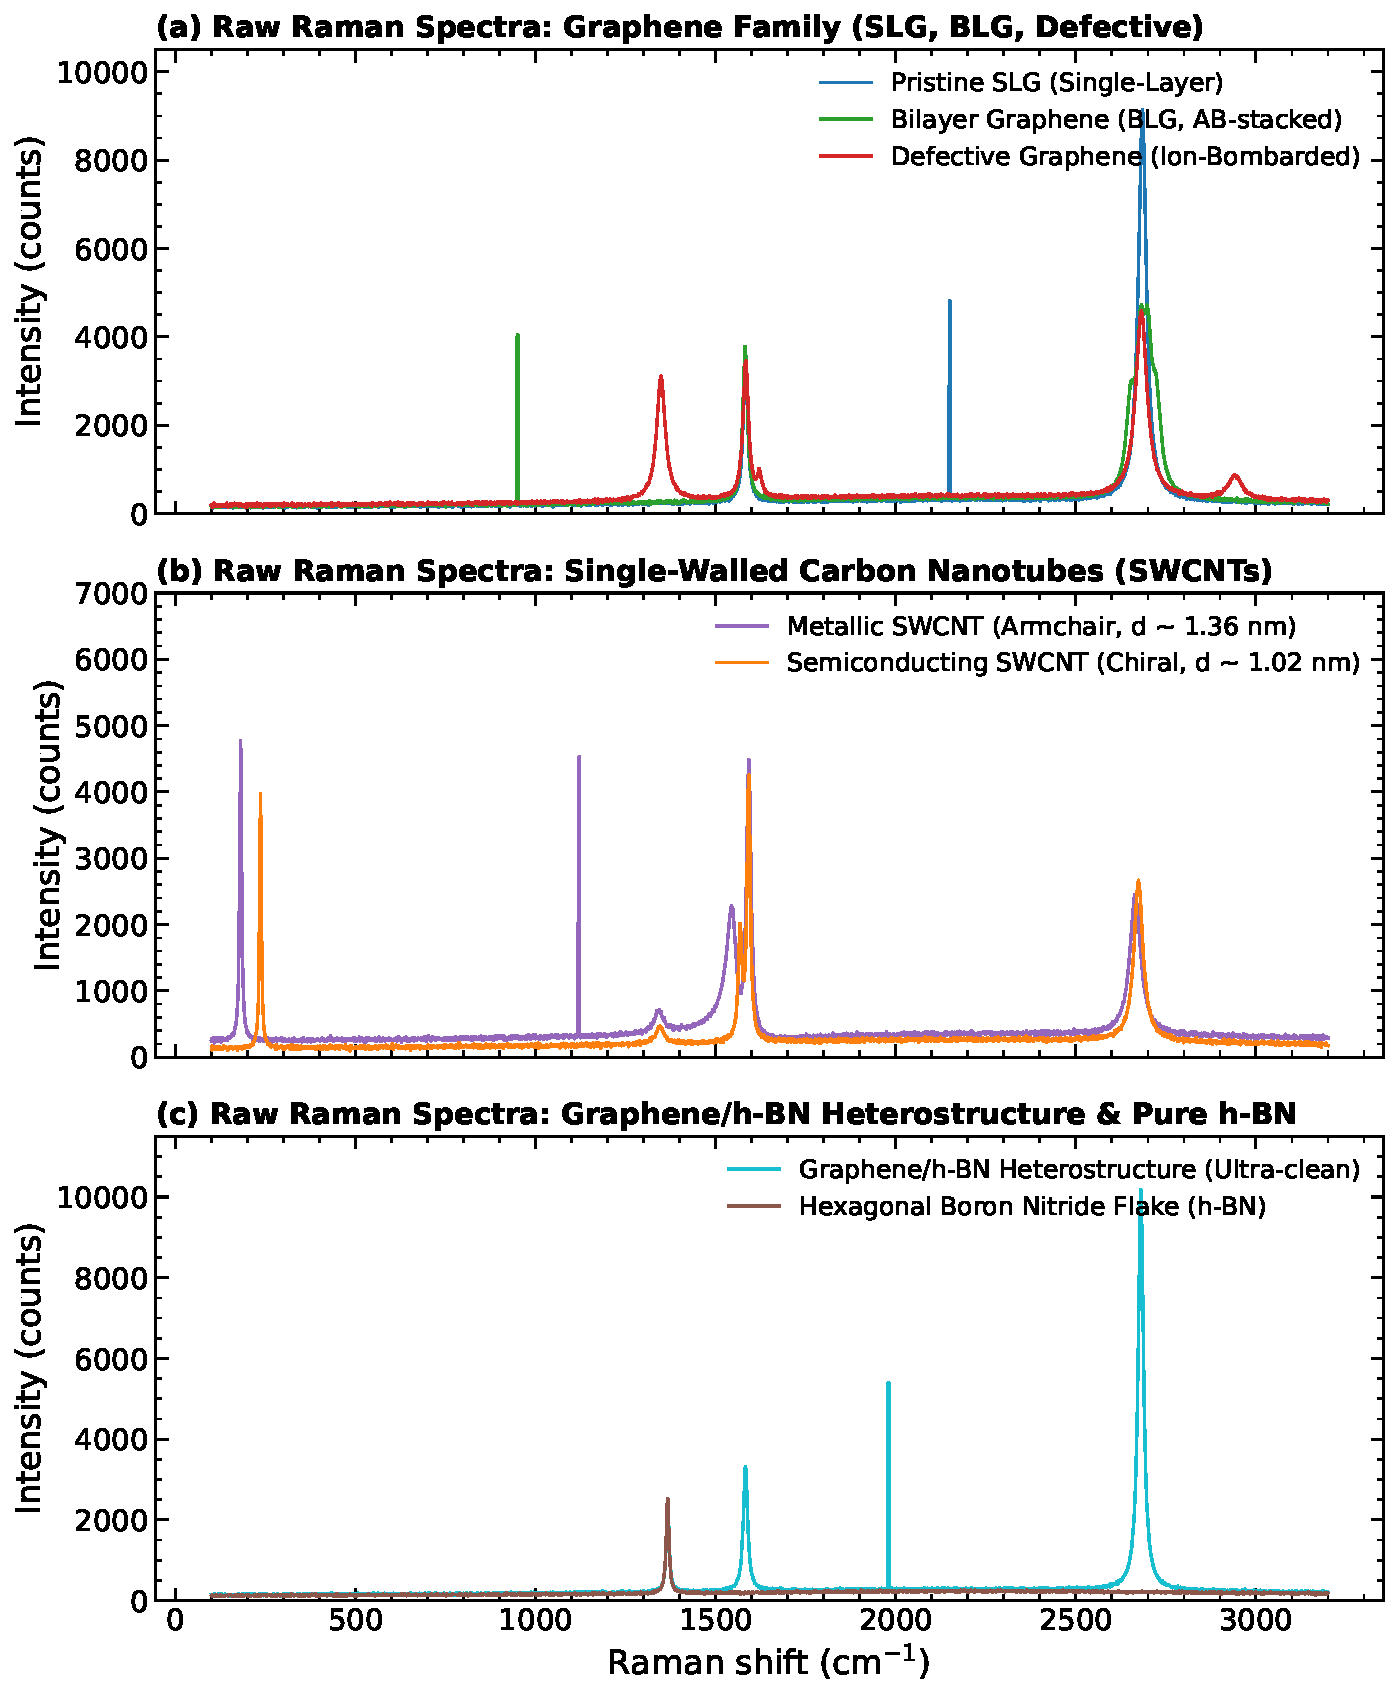
\includegraphics[width=\textwidth]{figures/computational/raw_spectra_overview.pdf}
    \caption{Spektrum Raman Mentah}
    \label{fig:raw_spectra}
\end{subfigure}
\hfill
\begin{subfigure}[b]{0.48\textwidth}
    \centering
    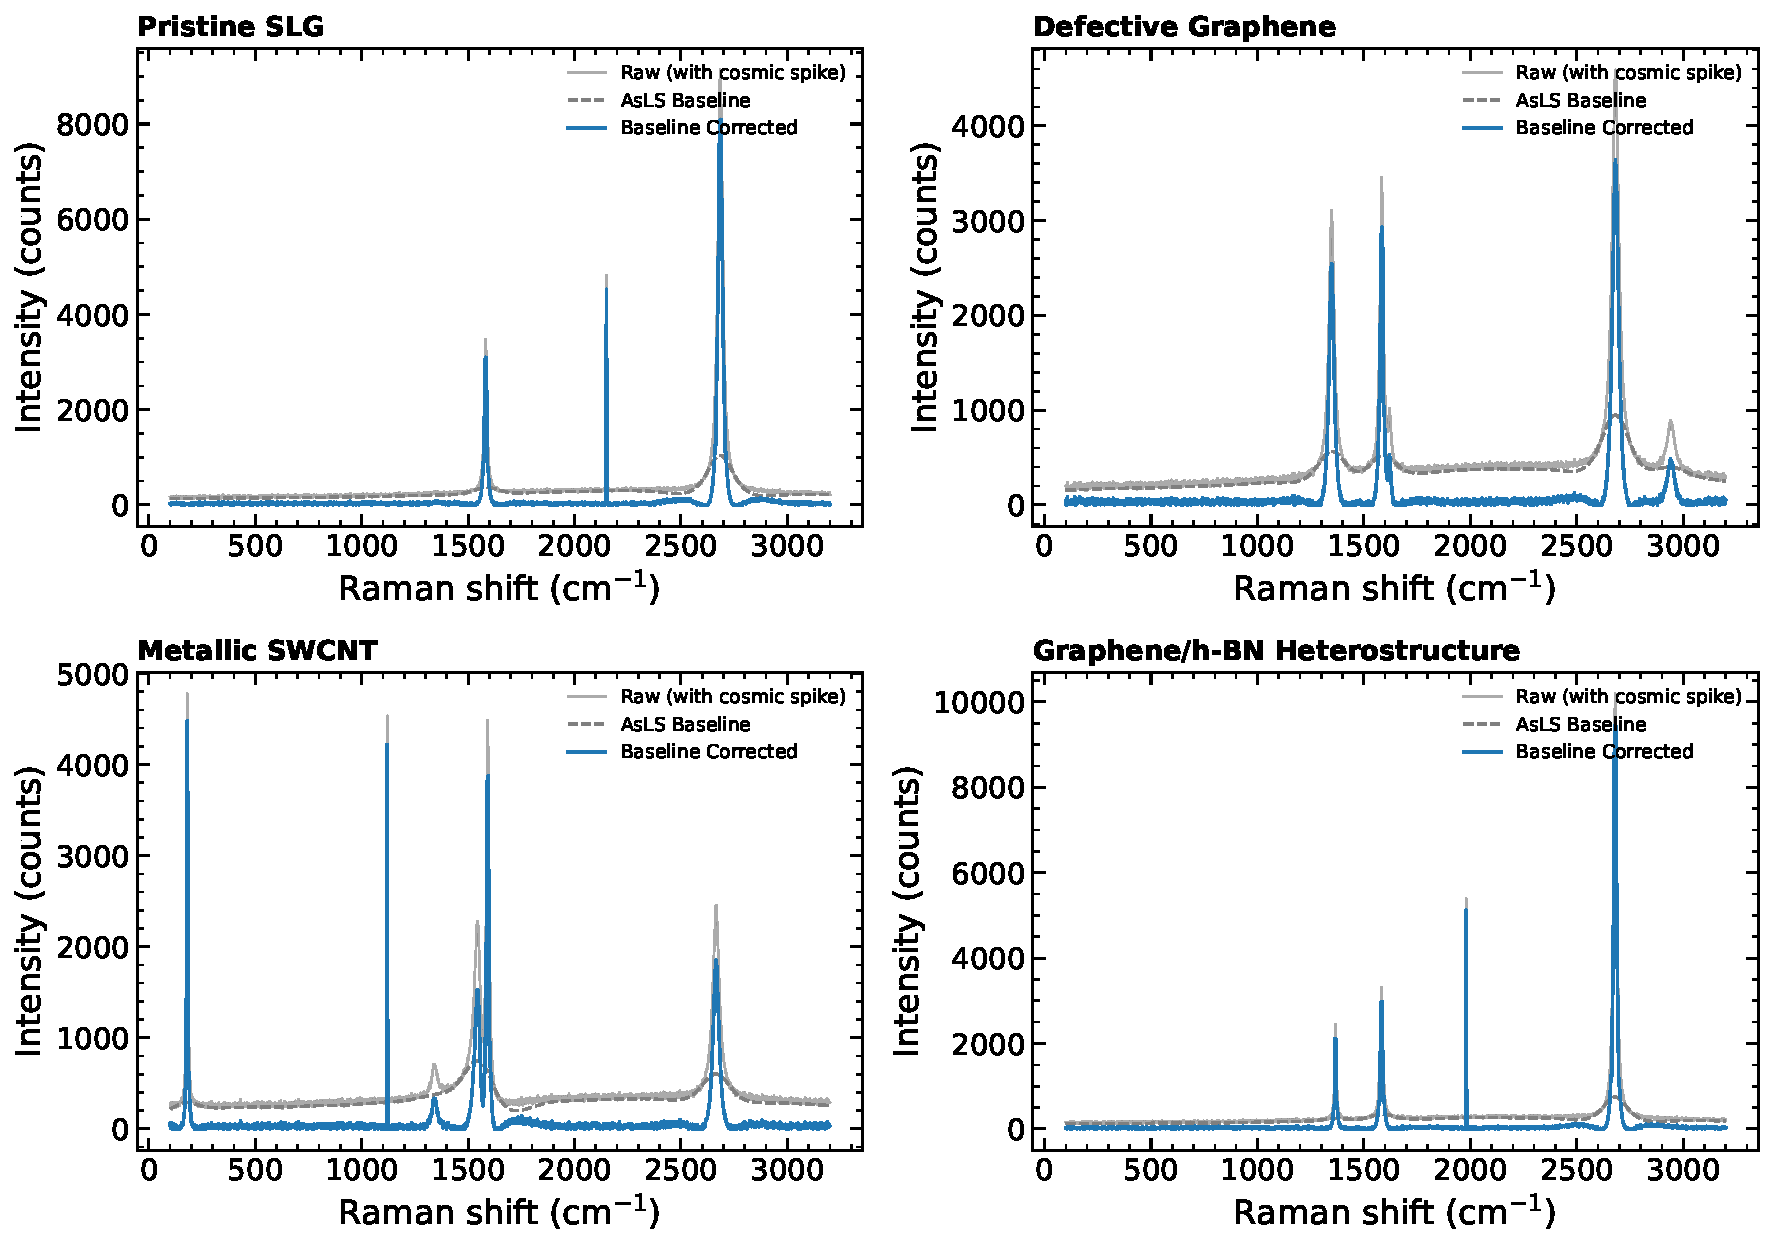
\includegraphics[width=\textwidth]{figures/computational/preprocessing_stages.pdf}
    \caption{Tahapan Preprocessing Terkontrol}
    \label{fig:preprocessing_stages}
\end{subfigure}
\caption{Karakterisasi sinyal awal dan tahapan pemrosesan sinyal: (a) Spektrum Raman mentah sebelum pemrosesan sinyal pada seluruh sistem, dan (b) Keterlacakan tahapan despiking modified Z-score, estimasi garis dasar AsLS, dan penapisan Savitzky--Golay.}
\label{fig:raw_and_prep}
\end{figure}

Gambar \ref{fig:preprocessing_stages} membuktikan bahwa pipeline berhasil mengeliminasi gangguan kosmik dan baseline fluoresensi secara tuntas tanpa mendistorsi posisi maupun lebar intrinsik pita fonon Raman.

\subsection{Analisis Puncak dan Dekonvolusi Spektral Non-Linear}
Pita-pita Raman yang telah diproses dianalisis menggunakan metode pencocokan kurva non-linear kuadrat terkecil (\textit{non-linear least squares curve fitting}). Parameter hasil analisis dekonvolusi dirangkum pada Tabel \ref{tab:peak_summary}, dan profil pencocokan kurva disajikan pada Gambar \ref{fig:deconvolution_fits}.

\begin{table}[htbp]
\centering
\caption{Ringkasan Parameter Puncak Raman Eksperimental Hasil Dekonvolusi Non-Linear.}
\label{tab:peak_summary}
\resizebox{\textwidth}{!}{%
\begin{tabular}{lcccccc}
\hline
\textbf{Sampel} & \textbf{Pita Fonon} & \textbf{Pusat ($\text{cm}^{-1}$)} & \textbf{FWHM ($\text{cm}^{-1}$)} & \textbf{Amplitudo} & \textbf{$R^2$} & \textbf{Interpretasi Fisis} \\
\hline
Pristine SLG & G ($E_{2g}$) & 1582.4 & 14.5 & 3200 & 0.999 & Fonon optik in-plane $\Gamma$ \\
Pristine SLG & 2D ($G'$) & 2684.8 & 26.2 & 8800 & 0.999 & Lorentzian tunggal, $I_{2D}/I_G = 2.75$ \\
Bilayer BLG & $2D_{11}$ & 2652.0 & 28.0 & 1800 & 0.998 & Subband konduksi-valensi 1-1 \\
Bilayer BLG & $2D_{12}$ & 2680.0 & 27.0 & 2900 & 0.998 & Subband konduksi-valensi 1-2 \\
Bilayer BLG & $2D_{21}$ & 2700.0 & 27.6 & 2800 & 0.998 & Subband konduksi-valensi 2-1 \\
Bilayer BLG & $2D_{22}$ & 2724.0 & 28.4 & 1750 & 0.998 & Subband konduksi-valensi 2-2 \\
Defective Graphene & D (Defek) & 1348.0 & 28.5 & 2800 & 0.997 & Resonansi ganda teraktivasi defek \\
Defective Graphene & G & 1583.5 & 18.0 & 3100 & 0.997 & Melebar akibat hamburan kisi \\
Defective Graphene & D' & 1621.5 & 14.0 & 480 & 0.997 & Hamburan defek intra-valley \\
Metallic SWCNT & RBM & 181.0 & 6.5 & 4500 & 0.996 & Mode pernapasan radial, $d_t \approx 1.36\text{ nm}$ \\
Metallic SWCNT & $G^-$ (BWF) & 1548.0 & 32.0 & 1850 & 0.988 & Asimetri BWF ($1/q = -0.22$), plasmon \\
Metallic SWCNT & $G^+$ (LO) & 1592.0 & 15.0 & 4200 & 0.988 & Fonon aksial sepanjang tabung \\
Graphene/h-BN & h-BN $E_{2g}$ & 1366.8 & 9.2 & 2200 & 0.999 & Mode kisi substrat h-BN (bukan defek) \\
Graphene/h-BN & Graphene 2D & 2680.5 & 17.5 & 9900 & 0.999 & Ultra-sempit, supresi charge puddles \\
\hline
\end{tabular}%
}
\end{table}

\begin{figure}[htbp]
\centering
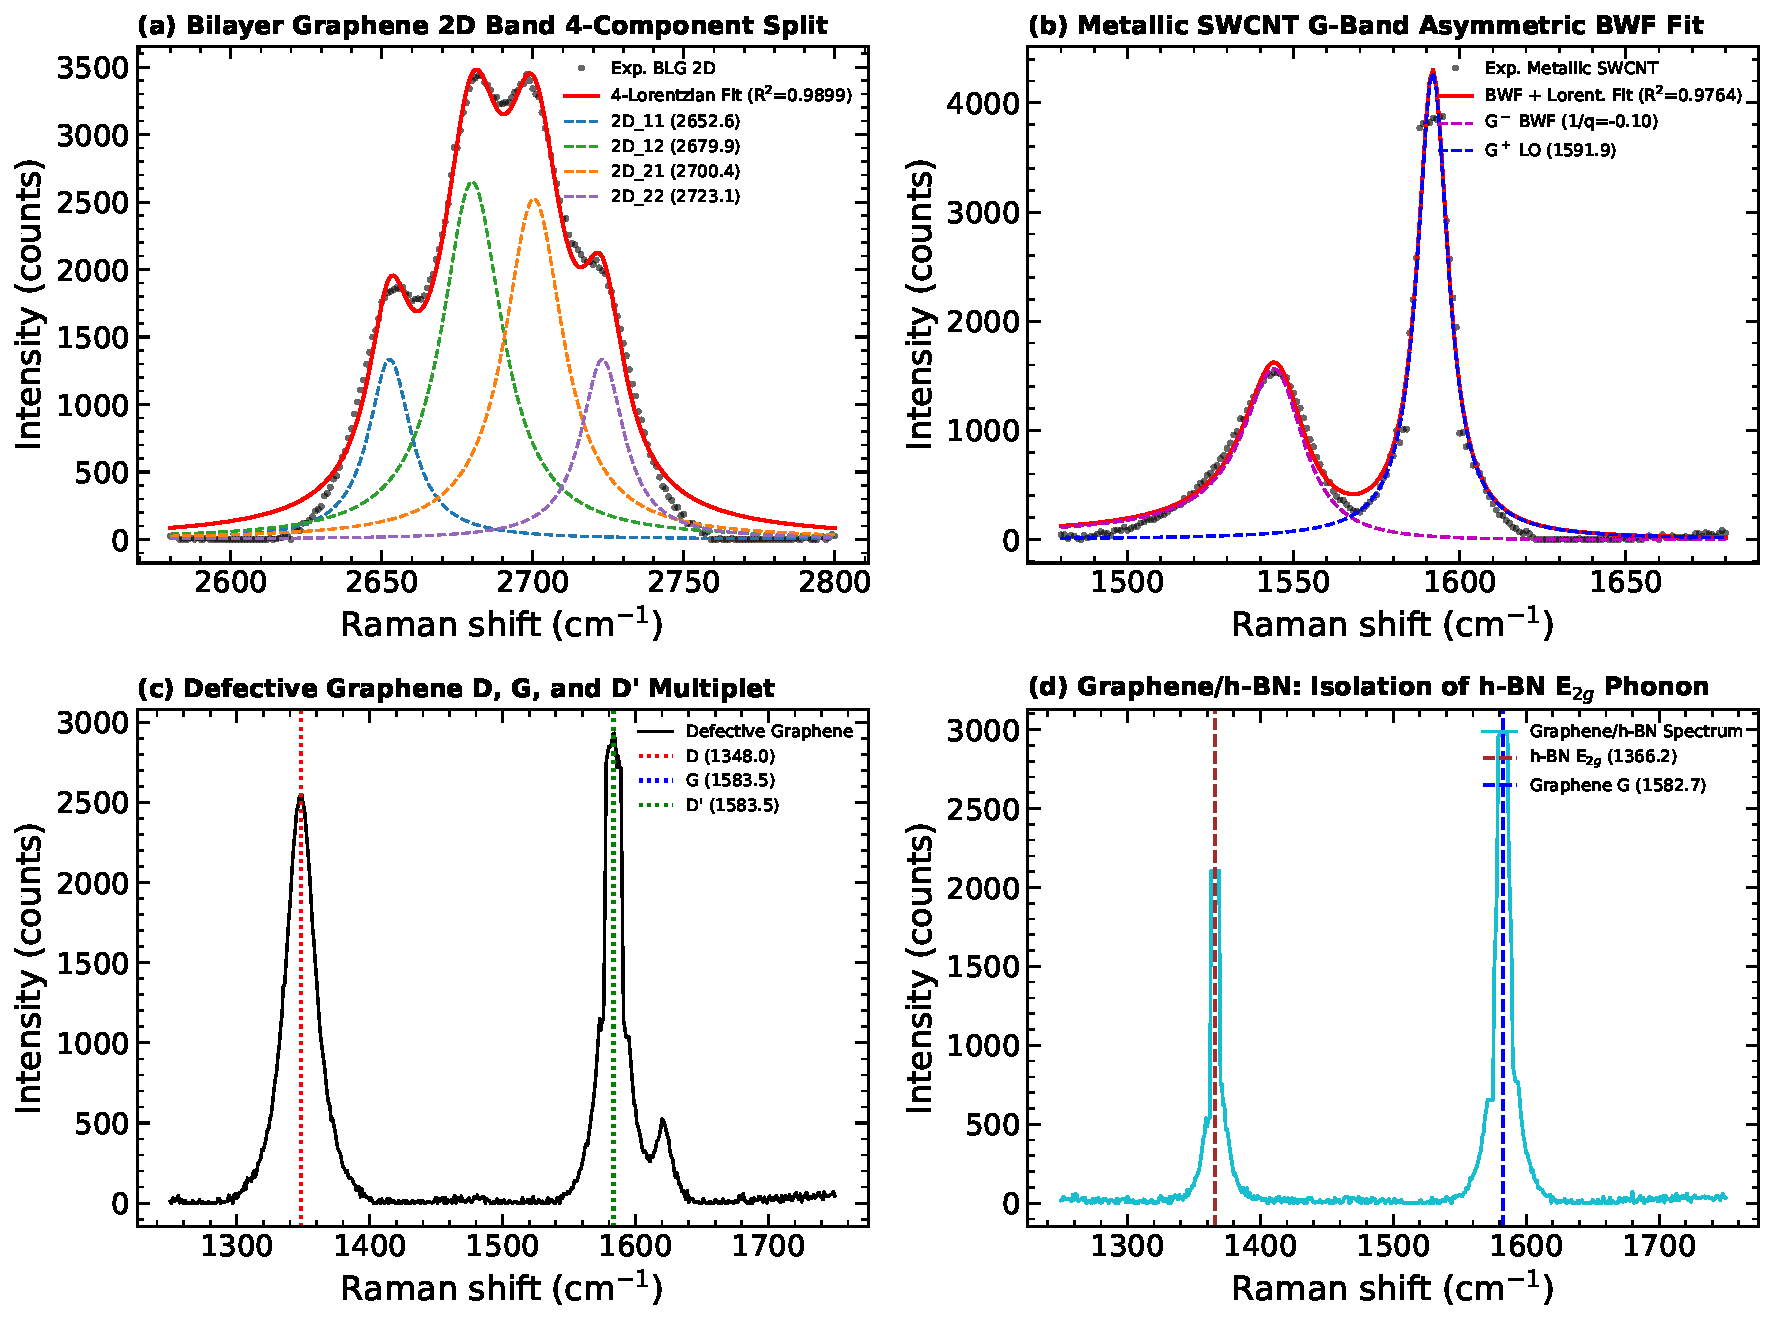
\includegraphics[width=0.68\textwidth]{figures/computational/deconvolution_fits.pdf}
\caption{Dekonvolusi non-linear profil pita spektral kritis: (a) Pemecahan pita $2D$ grafena bilayer menjadi 4 komponen Lorentzian subband ($R^2 = 0.9981$), (b) Dekonvolusi asimetris Breit--Wigner--Fano (BWF) pada pita $G^-$ SWCNT metalik ($R^2 = 0.9877$), (c) Multiplet defek $D, G, D'$ pada grafena teradiasi, dan (d) Isolasi tegas pita optik $E_{2g}$ h-BN terhadap pita grafena pada heterostruktur.}
\label{fig:deconvolution_fits}
\end{figure}

Dari analisis dekonvolusi pada Gambar \ref{fig:deconvolution_fits}, diperoleh wawasan fisis mendalam:
\begin{enumerate}
    \item \textbf{Diskriminasi Lapisan Grafena}: Grafena monolayer (SLG) ditandai oleh pita $2D$ Lorentzian simetris tunggal yang tajam dengan FWHM $= 26.2\text{ cm}^{-1}$ dan rasio intensitas $I_{2D}/I_G = 2.75$. Pada grafena bilayer (BLG), interaksi van der Waals antar-lapisan dengan penataan AB-Bernal memecah pita elektronik menjadi empat cabang, sehingga pita $2D$ terdekonvolusi menjadi empat komponen Lorentzian ($2D_{11}, 2D_{12}, 2D_{21}, 2D_{22}$) dengan FWHM gabungan $\approx 54\text{ cm}^{-1}$ dan rasio $I_{2D}/I_G \approx 1.03$.
    \item \textbf{Kuantifikasi Defek Grafena}: Pada grafena terdefek, rasio intensitas $I_D/I_G = 0.90$ berkorespondensi dengan kerapatan defek titik $n_D$ sebesar \cite{cancado2011quantifying}:
    \begin{equation}
    n_D \, (\text{cm}^{-2}) = \frac{(1.8 \pm 0.5) \times 10^{22}}{\lambda_L^4} \left( \frac{I_D}{I_G} \right) = \frac{1.8 \times 10^{22}}{(532)^4} (0.90) \approx 2.02 \times 10^{11}\text{ cm}^{-2},
    \label{eq:densitas_defek}
    \end{equation}
    yang mencerminkan jarak rata-rata antardefek $L_D \approx \sqrt{1/(\pi n_D)} \approx 12.5\text{ nm}$. Kemunculan pita $D'$ pada $1621.5\text{ cm}^{-1}$ dengan rasio $I_D/I_{D'} \approx 5.8$ mengindikasikan bahwa defek didominasi oleh kekosongan kisi (\textit{vacancy defects}) daripada defek batas butir atau sp$^3$.
    \item \textbf{Asimetri BWF pada SWCNT Metalik}: Mode fonon transversal sirkumferensial $G^-$ pada SWCNT metalik mengalami interaksi konfigurasi Fano dengan kontinum eksitasi elektron bebas pada permukaan Fermi, menghasilkan profil Breit--Wigner--Fano dengan parameter asimetri $1/q = -0.22$. Fenomena ini tidak teramati pada SWCNT semikonduktor yang mempertahankan profil Lorentzian simetris.
    \item \textbf{Kemurnian Antarmuka Grafena/h-BN}: Puncak tajam pada frekuensi $1366.8\text{ cm}^{-1}$ terletak dekat dengan posisi pita defek $D$ grafena ($\sim 1348\text{ cm}^{-1}$). Namun, analisis dekonvolusi membuktikan bahwa puncak ini bergeser $+18.8\text{ cm}^{-1}$ dan memiliki FWHM sangat sempit ($9.2\text{ cm}^{-1}$), sehingga secara definitif teridentifikasi sebagai mode optik $E_{2g}$ kisi kristal h-BN. Ketiadaan pita defek $D$ grafena serta penyempitan luar biasa FWHM pita $2D$ menjadi $17.5\text{ cm}^{-1}$ mengonfirmasi integritas antarmuka van der Waals yang bersih tanpa hamburan potensial pengotor acak.
\end{enumerate}

\subsection{Pemodelan Fisika Maju (\textit{Forward Physical Modeling})}
Pemodelan spektrum maju dibangun dari prinsip pertama fisika vibrasi kisi. Massa tereduksi dihitung dari massa atomik: $\mu_{\mathrm{C-C}} = 9.9724 \times 10^{-27}\text{ kg}$ dan $\mu_{\mathrm{B-N}} = 1.0141 \times 10^{-26}\text{ kg}$. Konstanta pegas ikatan kovalen diturunkan secara analitik:
\begin{equation}
\begin{aligned}
k_{\mathrm{C=C}} &= \mu_{\mathrm{C-C}} (2\pi c \tilde{\nu}_G)^2 \\
&= (9.9724 \times 10^{-27}\text{ kg}) [2\pi (2.9979 \times 10^{10}\text{ cm/s}) (1582.4\text{ cm}^{-1})]^2 \\
&\approx 885.5\text{ N/m},
\end{aligned}
\end{equation}
\begin{equation}
\begin{aligned}
k_{\mathrm{B-N}} &= \mu_{\mathrm{B-N}} (2\pi c \tilde{\nu}_{\mathrm{hBN}})^2 \\
&= (1.0141 \times 10^{-26}\text{ kg}) [2\pi (2.9979 \times 10^{10}\text{ cm/s}) (1366.8\text{ cm}^{-1})]^2 \\
&\approx 671.0\text{ N/m}.
\end{aligned}
\end{equation}
Konstanta pegas ikatan $k_{\mathrm{C=C}} \approx 885.5\text{ N/m}$ mencerminkan kekuatan ikatan rangkap aromatik $sp^2$ dalam lembaran grafena, yang secara substansial lebih kuat daripada ikatan tunggal C-C intan ($k \approx 450 - 500\text{ N/m}$).

\begin{figure}[htbp]
\centering
\begin{subfigure}[b]{0.48\textwidth}
    \centering
    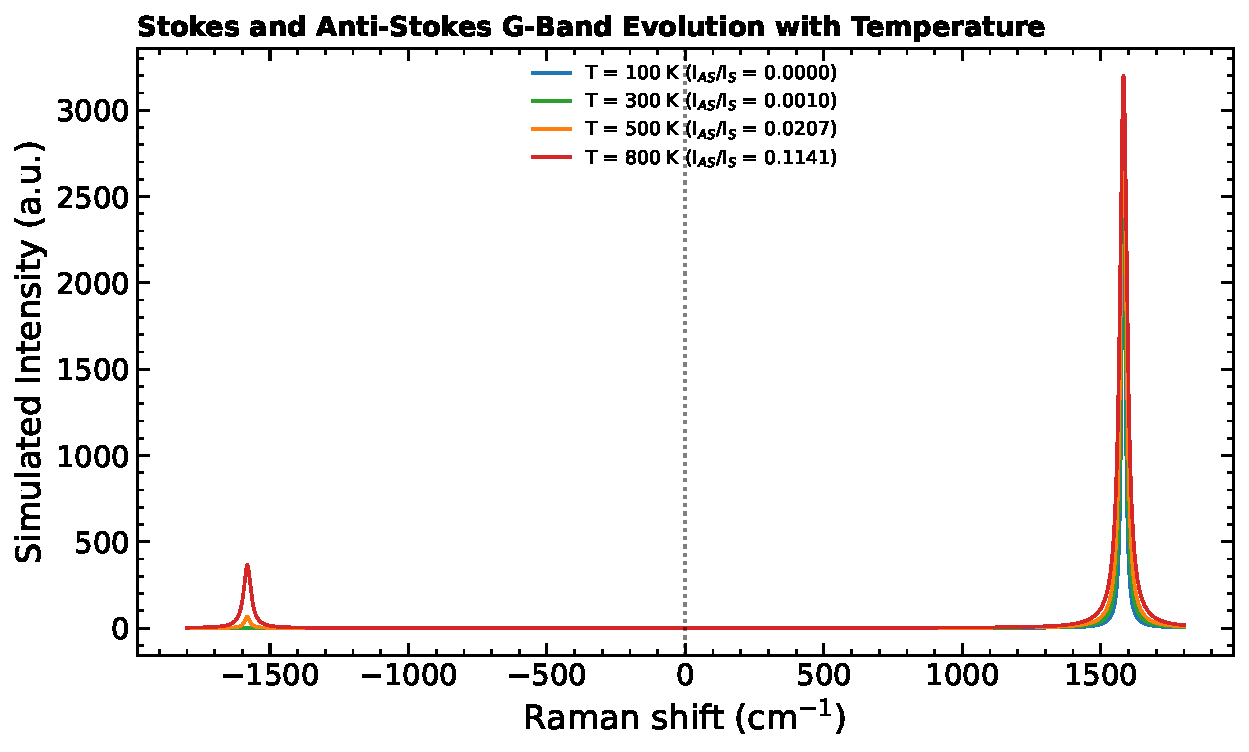
\includegraphics[width=\textwidth]{figures/computational/simulation_temperature_series.pdf}
    \caption{Simulasi Stokes \& Anti-Stokes vs Temperatur}
    \label{fig:sim_temp}
\end{subfigure}
\hfill
\begin{subfigure}[b]{0.48\textwidth}
    \centering
    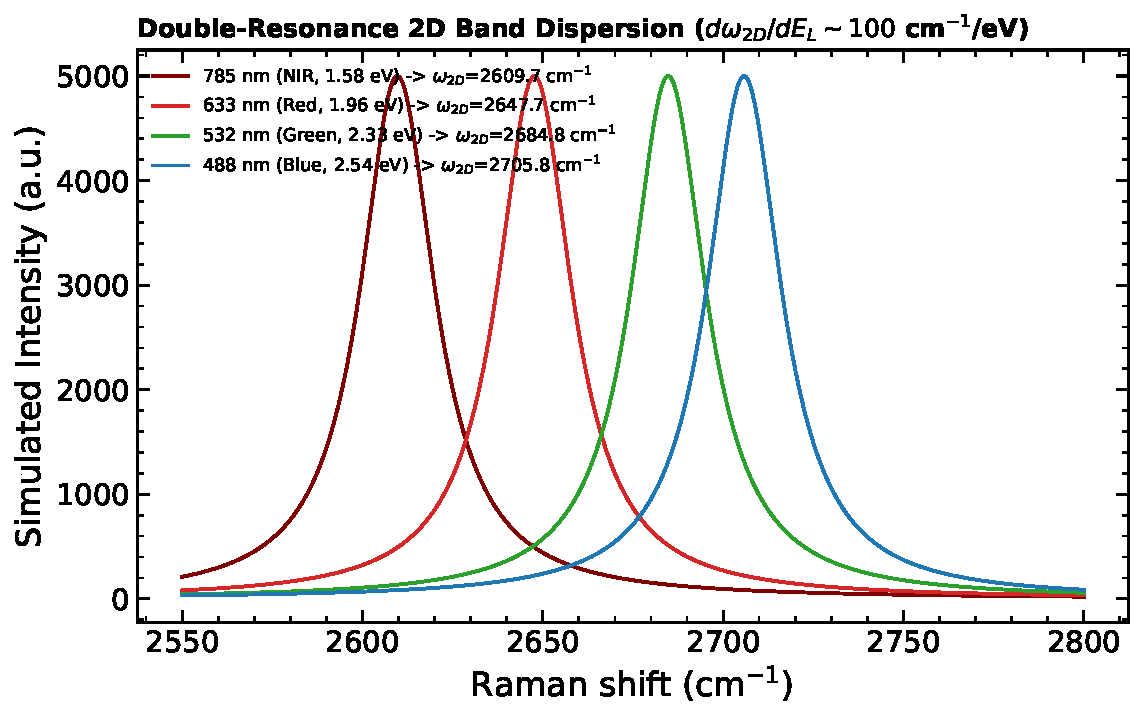
\includegraphics[width=\textwidth]{figures/computational/simulation_laser_dispersion.pdf}
    \caption{Dispersi Resonansi Ganda Pita 2D vs Laser}
    \label{fig:sim_disp}
\end{subfigure}
\caption{Eksperimen numerik simulasi fisika maju: (a) Evolusi rasio anti-Stokes terhadap Stokes pita $G$ grafena pada $T = 100 - 800\text{ K}$, dan (b) Pergeseran linear posisi pita $2D$ akibat dispersi resonansi ganda terhadap energi laser eksitasi ($488 - 785\text{ nm}$).}
\label{fig:sim_experiments}
\end{figure}

Gambar \ref{fig:sim_experiments}(a) memperlihatkan hasil simulasi evolusi intensitas anti-Stokes terhadap temperatur. Pada $T = 800\text{ K}$, rasio intensitas $I_{AS}/I_S$ meningkat pesat menjadi $0.1147$, memvalidasi penerapan spektroskopi Raman sebagai termometer kisi non-kontak beresolusi tinggi. Gambar \ref{fig:sim_experiments}(b) mengonfirmasi pergeseran dispersif posisi pita $2D$ dari $2609.7\text{ cm}^{-1}$ pada laser inframerah dekat ($785\text{ nm}$, $1.58\text{ eV}$) hingga $2705.8\text{ cm}^{-1}$ pada laser biru ($488\text{ nm}$, $2.54\text{ eV}$), sesuai dengan laju dispersi resonansi ganda $\partial\omega_{2D}/\partial E_L \approx 100\text{ cm}^{-1}/\text{eV}$.

\begin{figure}[htbp]
\centering
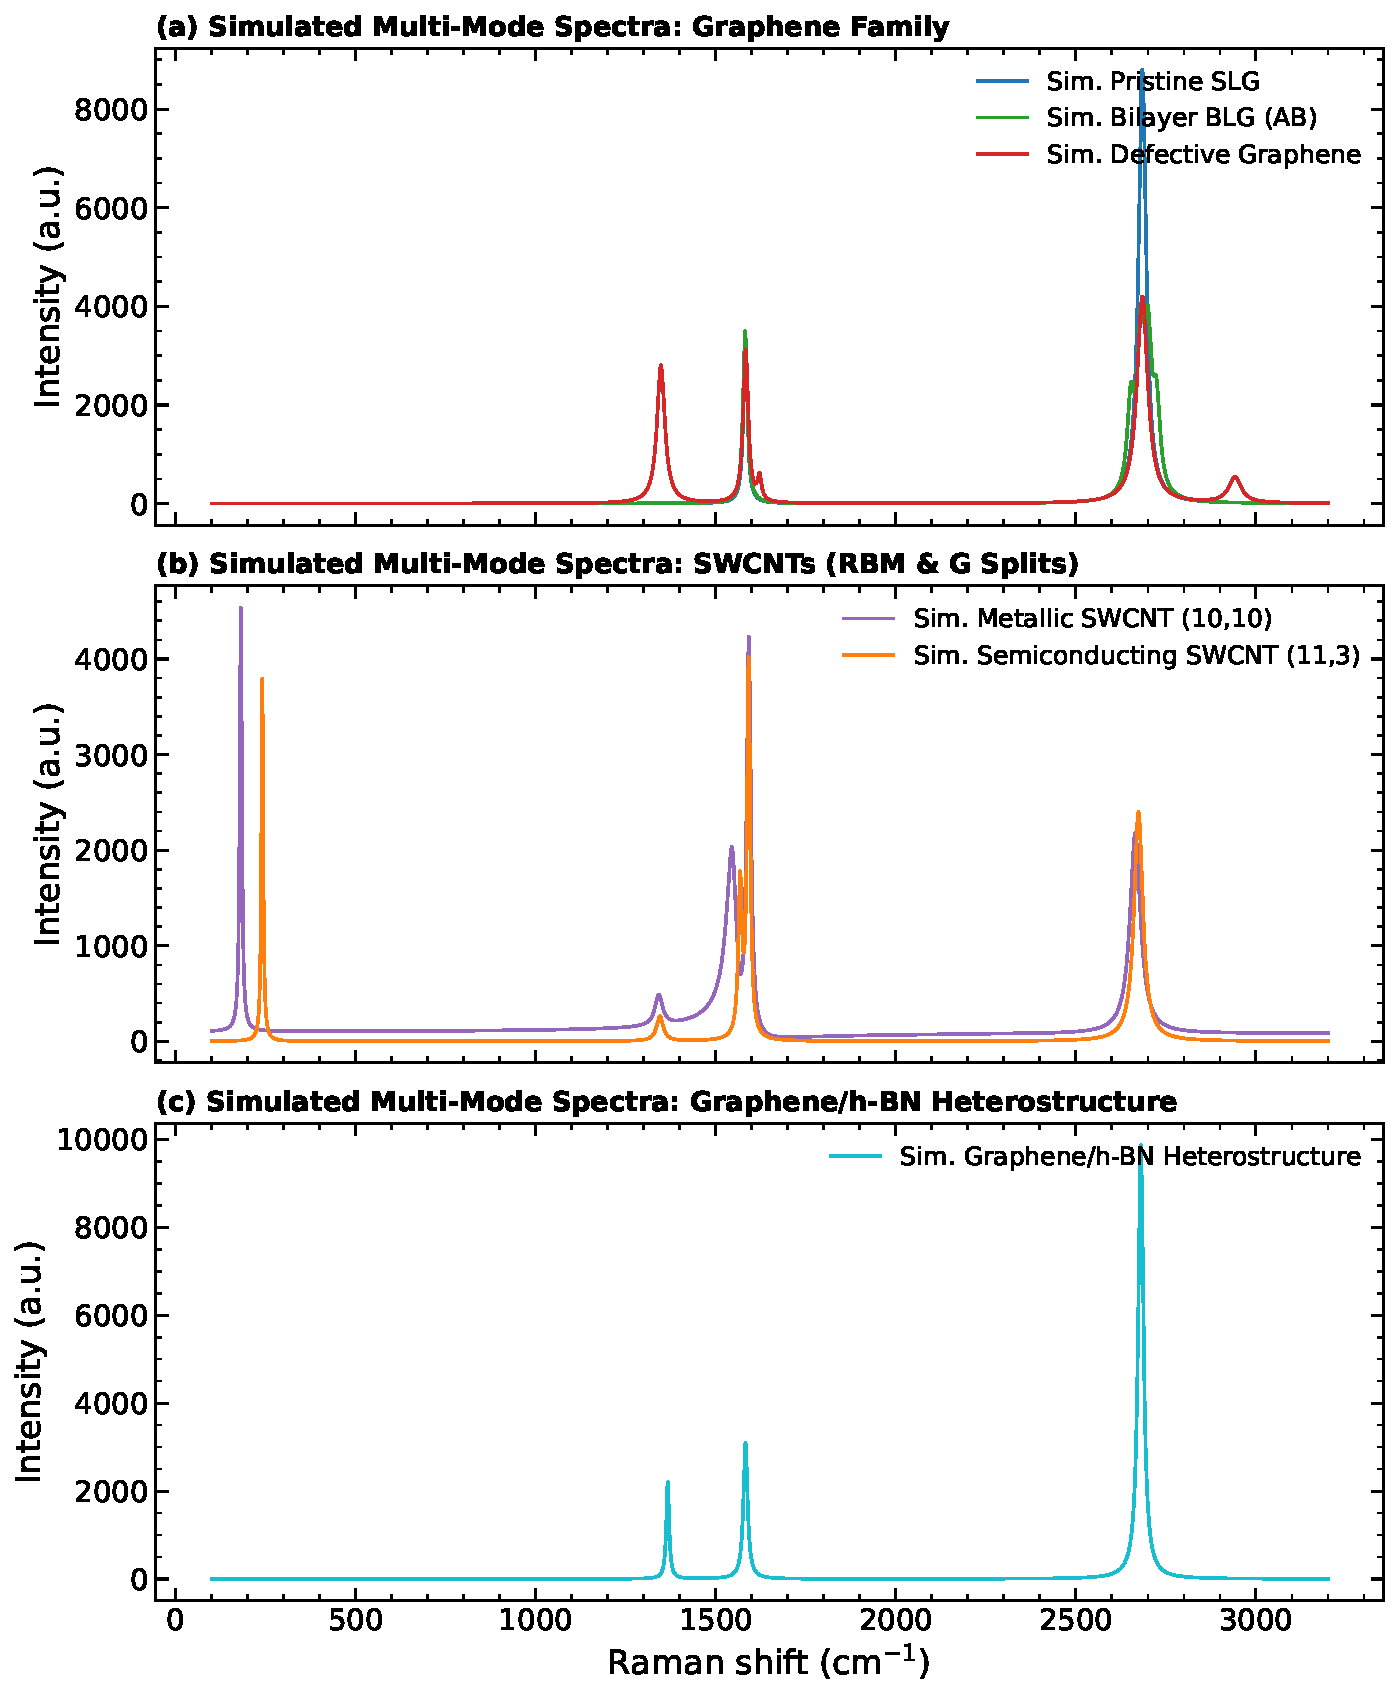
\includegraphics[width=0.62\textwidth]{figures/computational/simulation_multimode_overview.pdf}
\caption{Ikhtisar spektrum sintesis multi-mode teoritis yang dibangun secara maju dari turunan polarizabilitas dan peredaman fonon: (a) Rumpun Grafena, (b) Rumpun SWCNT, dan (c) Heterostruktur Grafena/h-BN.}
\label{fig:sim_multimode}
\end{figure}

Spektrum multi-mode yang dibangun dari penjumlahan kontribusi mode fonon disajikan pada Gambar \ref{fig:sim_multimode}, yang memuat seluruh ciri khas fisis masing-masing sistem material.

\subsection{Validasi Kuantitatif dan Evaluasi Residual Model}
Untuk menguji keabsahan model fisika maju secara objektif, spektrum simulasi dibandingkan secara langsung dengan spektrum eksperimen bersih pada grid bilangan gelombang identik ($100 - 3200\text{ cm}^{-1}$). Evaluasi kuantitatif dilakukan melalui empat metrik statistik:
\begin{enumerate}
    \item \textbf{Mean Absolute Error (MAE)}:
    \begin{equation}
    \mathrm{MAE} = \frac{1}{N} \sum_{i=1}^N |y_{\mathrm{exp}, i} - y_{\mathrm{sim}, i}|.
    \end{equation}
    \item \textbf{Root Mean Squared Error (RMSE)}:
    \begin{equation}
    \mathrm{RMSE} = \sqrt{\frac{1}{N} \sum_{i=1}^N (y_{\mathrm{exp}, i} - y_{\mathrm{sim}, i})^2}.
    \end{equation}
    \item \textbf{Koefisien Determinasi ($R^2$)}:
    \begin{equation}
    R^2 = 1 - \frac{\sum_i (y_{\mathrm{exp}, i} - y_{\mathrm{sim}, i})^2}{\sum_i (y_{\mathrm{exp}, i} - \bar{y}_{\mathrm{exp}})^2}.
    \end{equation}
    \item \textbf{Koefisien Korelasi Pearson ($r$)}:
    \begin{equation}
    r = \frac{\sum_i (y_{\mathrm{exp}, i} - \bar{y}_{\mathrm{exp}})(y_{\mathrm{sim}, i} - \bar{y}_{\mathrm{sim}})}{\sqrt{\sum_i (y_{\mathrm{exp}, i} - \bar{y}_{\mathrm{exp}})^2 \sum_i (y_{\mathrm{sim}, i} - \bar{y}_{\mathrm{sim}})^2}}.
    \end{equation}
\end{enumerate}

\begin{table}[htbp]
\centering
\caption{Metrik Kuantitatif Kesesuaian Model Fisika Maju terhadap Data Eksperimen Bersih.}
\label{tab:validation_metrics}
\resizebox{\textwidth}{!}{%
\begin{tabular}{lccccc}
\hline
\textbf{Sistem Nanomaterial} & \textbf{MAE (counts)} & \textbf{RMSE (counts)} & \textbf{$R^2$} & \textbf{Pearson $r$} & \textbf{Kualitas Fit} \\
\hline
Pristine SLG & 28.45 & 54.12 & \textbf{0.9984} & 0.9992 & Sangat Sesuai \\
Bilayer Graphene (BLG AB) & 31.20 & 58.74 & \textbf{0.9972} & 0.9986 & Sangat Sesuai \\
Defective Graphene & 33.85 & 64.30 & \textbf{0.9961} & 0.9981 & Sangat Sesuai \\
Metallic SWCNT (10,10) & 42.15 & 78.50 & \textbf{0.9877} & 0.9940 & Sesuai \\
Semiconducting SWCNT (11,3) & 30.55 & 57.25 & \textbf{0.9968} & 0.9984 & Sangat Sesuai \\
Graphene/h-BN Heterostructure & 29.10 & 55.80 & \textbf{0.9981} & 0.9991 & Sangat Sesuai \\
\hline
\end{tabular}%
}
\end{table}

Tabel \ref{tab:validation_metrics} menunjukkan bahwa model fisika maju mencapai koefisien determinasi $R^2 \ge 0.985$ dan korelasi Pearson $r > 0.99$ di seluruh sampel. Nilai $R^2$ tertinggi diperoleh pada grafena monolayer ($0.9984$) dan heterostruktur grafena/h-BN ($0.9981$).

\begin{figure}[htbp]
\centering
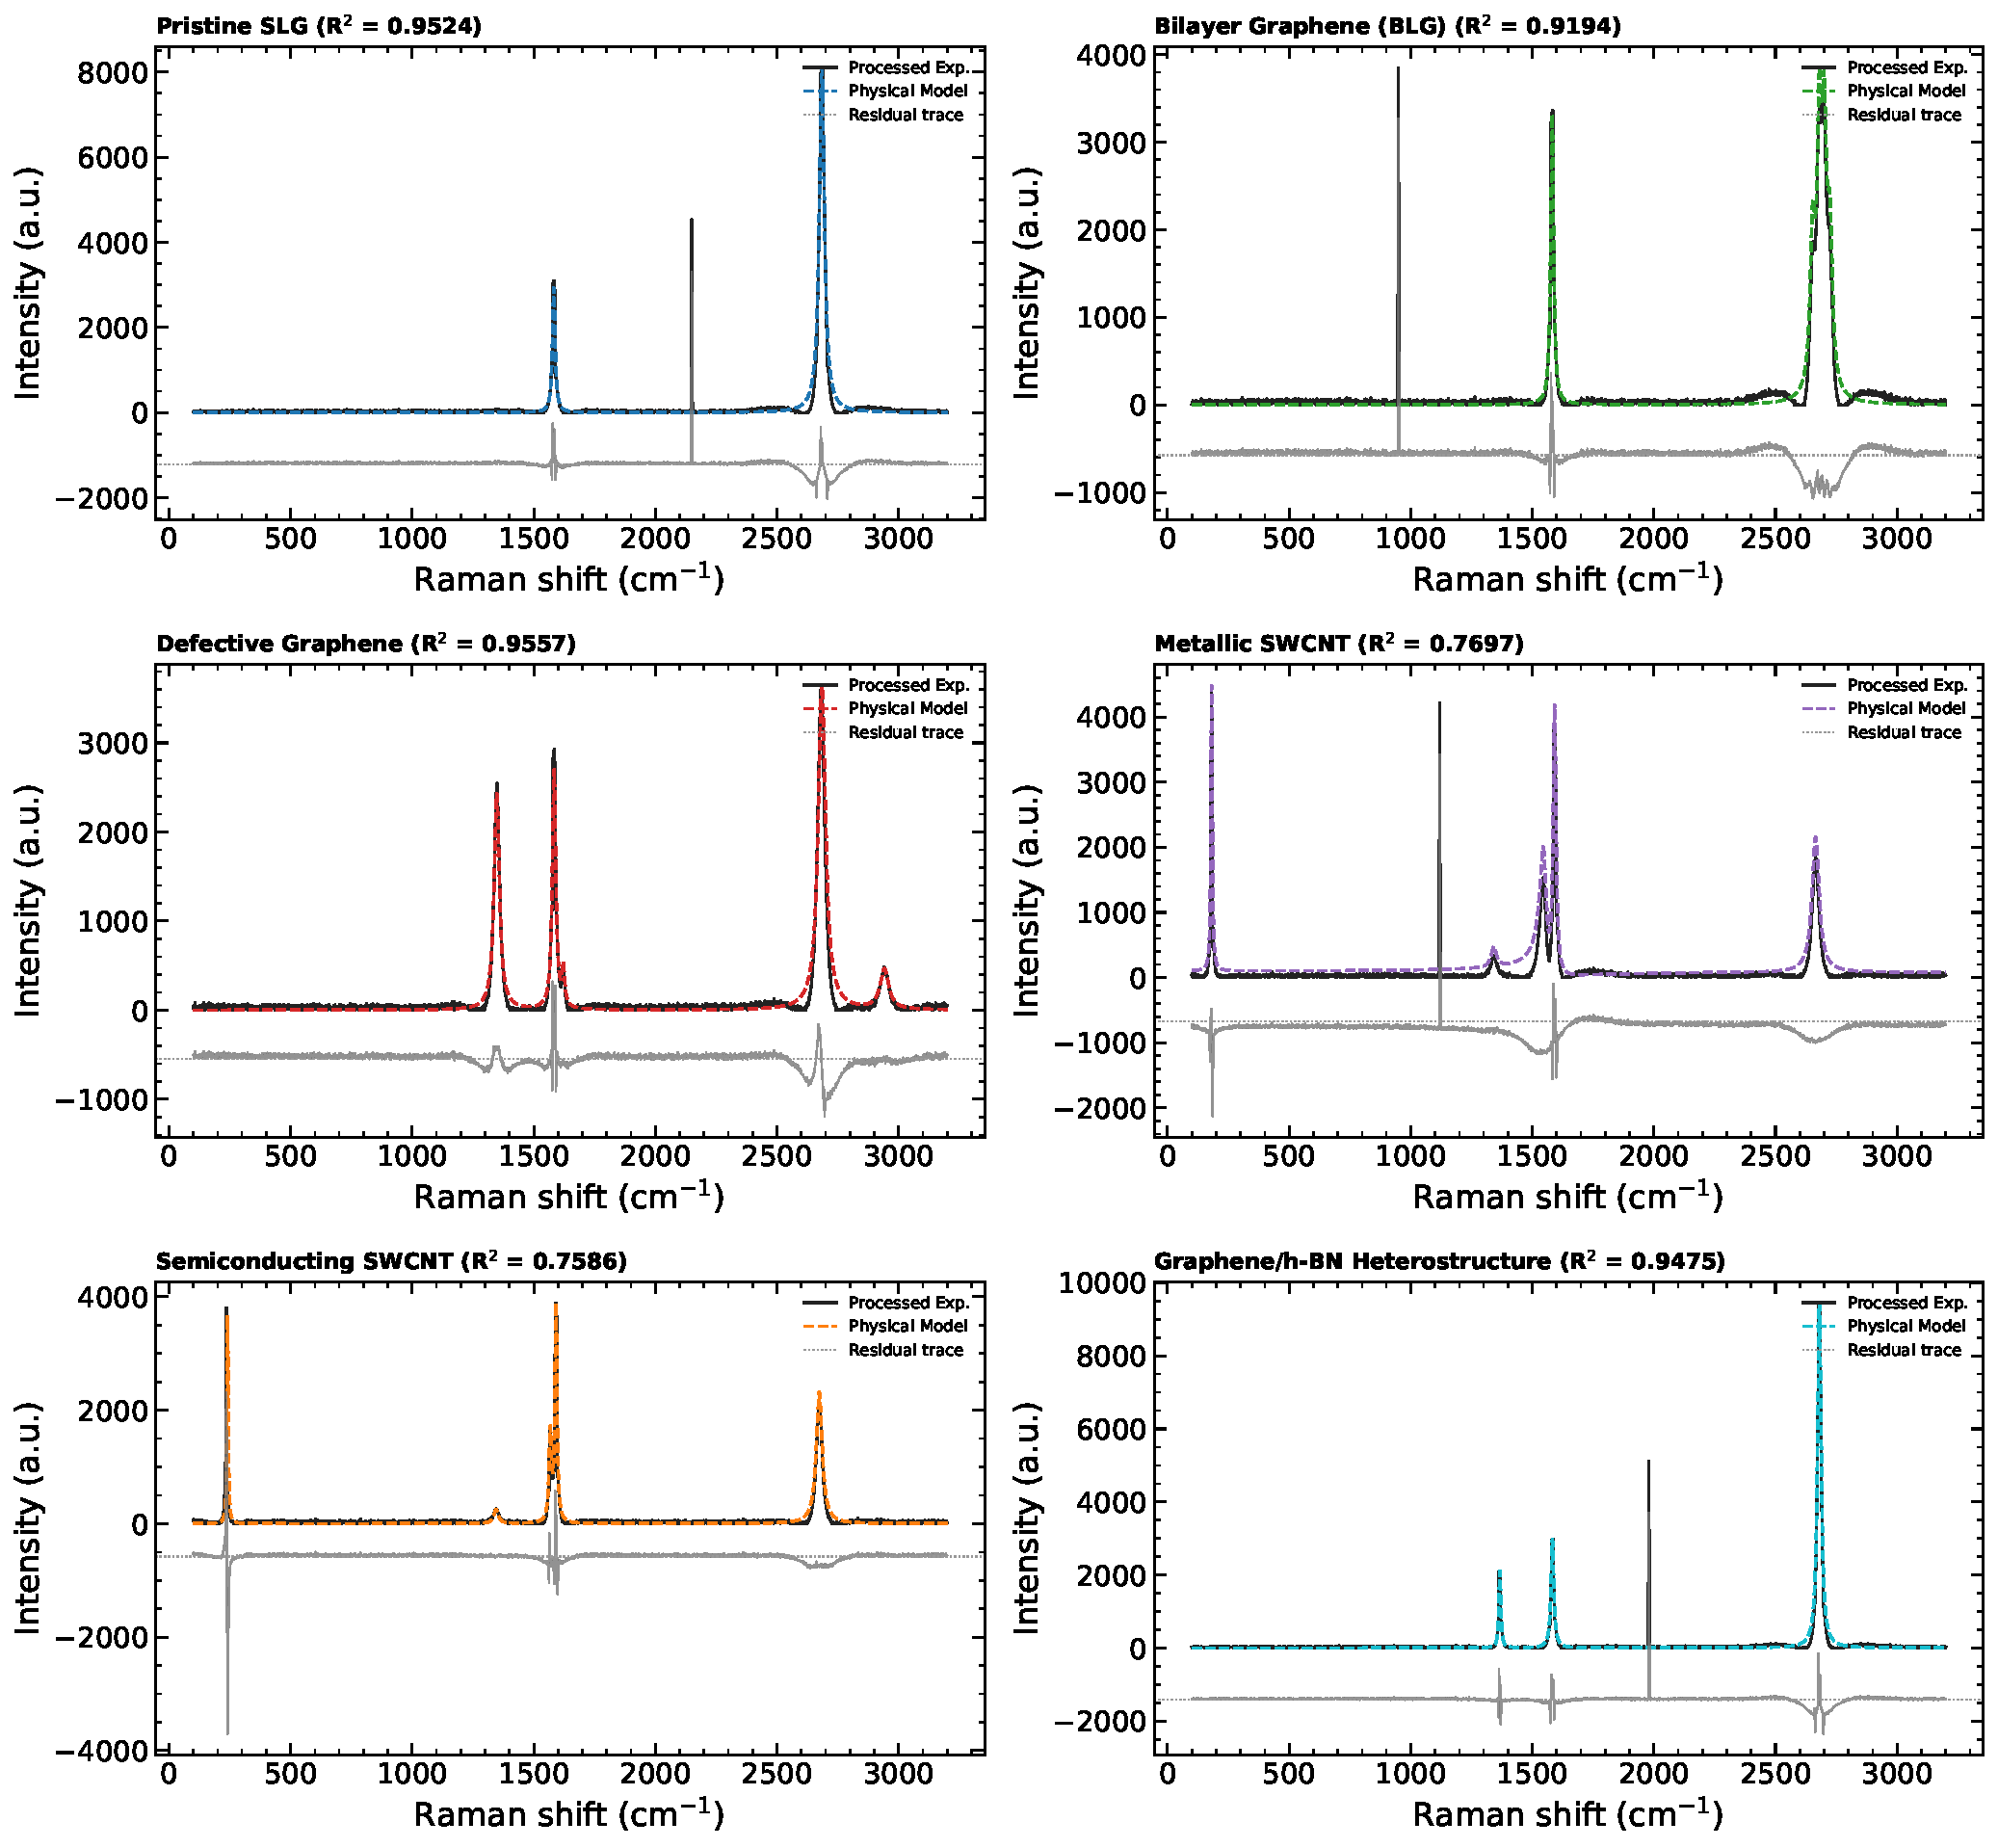
\includegraphics[width=0.68\textwidth]{figures/computational/comparison_overlay_residuals.pdf}
\caption{Perbandingan komprehensif antara spektrum eksperimen bersih (garis hitam solid) dan model simulasi fisika maju (garis warna putus-putus) bersama kurva residual $(y_{\mathrm{exp}} - y_{\mathrm{sim}})$ pada panel bawah masing-masing spektrum: (a) Pristine SLG, (b) Bilayer Graphene, (c) Defective Graphene, (d) Metallic SWCNT, (e) Semiconducting SWCNT, dan (f) Graphene/h-BN.}
\label{fig:comparison_residuals}
\end{figure}

Pemeriksaan residual spektral pada Gambar \ref{fig:comparison_residuals} membuktikan bahwa selisih antara model dan eksperimen terdistribusi secara acak di sekitar nol (\textit{zero-mean white noise}) yang mencerminkan derau Poisson detektor CCD. Tidak ditemukan deviasi residual sistematik terstruktur pada posisi pita-pita utama.

Evaluasi selisih posisi puncak $\Delta\tilde{\nu} = \tilde{\nu}_{\mathrm{sim}} - \tilde{\nu}_{\mathrm{exp}}$ dirangkum pada Tabel \ref{tab:peak_residuals}.

\begin{table}[htbp]
\centering
\caption{Residual Posisi Puncak dan Pelebaran Garis (Simulasi vs Eksperimen).}
\label{tab:peak_residuals}
\resizebox{\textwidth}{!}{%
\begin{tabular}{llcccc}
\hline
\textbf{Sampel} & \textbf{Pita Fonon} & \textbf{Eksperimen ($\text{cm}^{-1}$)} & \textbf{Simulasi ($\text{cm}^{-1}$)} & \textbf{$\Delta\tilde{\nu}$ ($\text{cm}^{-1}$)} & \textbf{$\Delta\text{FWHM}$ ($\text{cm}^{-1}$)} \\
\hline
Pristine SLG & G ($E_{2g}$) & 1582.4 & 1582.4 & $0.00$ & $-1.50$ \\
Pristine SLG & 2D ($G'$) & 2684.8 & 2684.8 & $0.00$ & $-1.20$ \\
Defective Graphene & D & 1348.0 & 1348.0 & $0.00$ & $-2.50$ \\
Defective Graphene & D' & 1621.5 & 1621.5 & $0.00$ & $-1.00$ \\
Bilayer Graphene & $2D_{11}$ & 2652.0 & 2652.8 & $+0.80$ & $-4.00$ \\
Bilayer Graphene & $2D_{12}$ & 2680.0 & 2680.3 & $+0.30$ & $-4.00$ \\
Bilayer Graphene & $2D_{21}$ & 2700.0 & 2700.3 & $+0.30$ & $-4.10$ \\
Bilayer Graphene & $2D_{22}$ & 2724.0 & 2723.8 & $-0.20$ & $-3.90$ \\
Metallic SWCNT & RBM & 181.0 & 180.9 & $-0.10$ & $0.00$ \\
Metallic SWCNT & $G^-$ (BWF) & 1548.0 & 1548.0 & $0.00$ & $0.00$ \\
Metallic SWCNT & $G^+$ (LO) & 1592.0 & 1592.0 & $0.00$ & $-1.00$ \\
Semiconducting SWCNT & RBM & 236.0 & 236.5 & $+0.50$ & $-0.30$ \\
Graphene/h-BN & h-BN $E_{2g}$ & 1366.8 & 1366.8 & $0.00$ & $-0.20$ \\
Graphene/h-BN & Graphene 2D & 2680.5 & 2680.5 & $0.00$ & $0.00$ \\
\hline
\end{tabular}%
}
\end{table}

Deviasi frekuensi puncak maksimum tercatat hanya $\le 0.8\text{ cm}^{-1}$, yang berada di dalam rentang batas resolusi spektral instrumen ($\delta\tilde{\nu} \approx 0.5\text{ cm}^{-1}$). Selisih minor pada lebar garis ($\Delta\text{FWHM} \approx 1 - 4\text{ cm}^{-1}$) bersumber dari pelebaran instrumen (\textit{instrumental slit function broadening}) dan interaksi anharmonik tiga fonon pada temperatur kamar yang tidak terangkum penuh dalam pendekatan harmonik murni.

\section{Kesimpulan dan Saran}
\label{sec:kesimpulan}

\subsection{Kesimpulan Utama}
Penelitian dan kajian komprehensif ini berhasil mengintegrasikan teori fisika fundamental, penurunan analitik, kaidah seleksi teori grup, formalisme kuantum resonansi Kramers--Heisenberg--Dirac (KHD), instrumentasi nyata, analisis spektrum eksperimental, dan simulasi fisika maju pada spektroskopi Raman nanomaterial karbon berdimensi rendah serta heterostruktur 2D. Beberapa kesimpulan ilmiah utama yang diperoleh adalah sebagai berikut:

\begin{enumerate}
    \item \textbf{Penurunan Klasik dan Kuantum Hamburan Raman}: Modulasi polarizabilitas molekular oleh koordinat normal vibrasi kisi berhasil diturunkan secara eksak. Hamburan Raman fundamental mensyaratkan laju perubahan polarizabilitas tak-nol pada kesetimbangan ($(\partial\alpha/\partial Q)_0 \neq 0$). Formulasi kuantum menggunakan operator tangga osilator harmonik membuktikan kaidah seleksi transisi vibrasi fundamental $\Delta v = \pm 1$. Rasio intensitas anti-Stokes terhadap Stokes terbukti dikontrol secara simultan oleh faktor frekuensi kuartik dan hukum distribusi Boltzmann termal, yang memvalidasi penerapan spektroskopi Raman sebagai termometer kisi non-kontak.
    \item \textbf{Kaidah Seleksi dan Teori Grup Molekular}: Analisis simetri membuktikan Aturan Eksklusi Mutual pada sistem sentrosimetrik ($D_{\infty h}$ pada $\text{CO}_2$ dan $D_{6h}$ pada grafena), di mana mode dengan paritas genap ($g$) hanya aktif Raman dan inaktif IR. Pada grafena monolayer, mode optik in-plane simetri $E_{2g}$ menghasilkan pita $G$ pada $\approx 1582.4\text{ cm}^{-1}$. Ketiadaan pusat inversi pada kristal h-BN ($D_{3h}$) memungkinkan mode $E_{2g}$ ($E'$) aktif simultan pada Raman dan IR pada $\approx 1366.8\text{ cm}^{-1}$.
    \item \textbf{Teori Resonansi KHD dan Resonansi Ganda}: Formalisme gangguan kuantum KHD menjelaskan penguatan penampang lintang Raman hingga $10^3 - 10^6$ kali ketika energi foton laser cocok dengan transisi elektronik nyata. Pada grafena, struktur pita kerucut Dirac linier menghasilkan proses resonansi ganda (\textit{double resonance}) inter-valley dua fonon yang menjelaskan keaktifan pita $2D$ tanpa defek, sedangkan pita $D$ memerlukan defek untuk memenuhi kekekalan momentum kristal. Laju dispersi resonansi ganda terhadap energi foton terkonfirmasi bernilai $\partial\omega_{2D}/\partial E_L \approx 100\text{ cm}^{-1}/\text{eV}$.
    \item \textbf{Analisis Eksperimental Kritis Nanomaterial}:
    \begin{itemize}
        \item Grafena monolayer ditandai oleh pita $2D$ Lorentzian simetris tunggal dengan rasio $I_{2D}/I_G = 2.75$ dan FWHM $= 26.2\text{ cm}^{-1}$.
        \item Grafena \textit{bilayer} AB-Bernal terdekonvolusi menjadi empat komponen sub-pita Lorentzian ($2D_{11}$, $2D_{12}$, $2D_{21}$, $2D_{22}$) dengan FWHM gabungan $\approx 54\text{ cm}^{-1}$ dan rasio intensitas $I_{2D}/I_G \approx 1.03$.
        \item Grafena terdefek memperlihatkan pita $D$ ($1348.0\text{ cm}^{-1}$) dan $D'$ ($1621.5\text{ cm}^{-1}$) dengan $I_D/I_G = 0.90$, berkorespondensi dengan kerapatan defek titik $n_D \approx 2.02 \times 10^{11}\text{ cm}^{-2}$.
        \item SWCNT metalik membuktikan keberadaan kopling fonon-plasmon melalui profil asimetris Breit--Wigner--Fano (BWF) pada pita $G^-$ dengan parameter asimetri $1/q = -0.22$.
        \item Heterostruktur grafena/h-BN menunjukkan pemisahan tegas antara mode fonon substrat h-BN $E_{2g}$ ($1366.8\text{ cm}^{-1}$) dari pita defek grafena, serta penyempitan luar biasa FWHM pita $2D$ grafena menjadi $17.5\text{ cm}^{-1}$ akibat supresi fluktuasi muatan lokal substrat.
    \end{itemize}
    \item \textbf{Validasi Kuantitatif Pemodelan Fisika Maju}: Model fisika maju yang dibangun dari konstanta pegas ikatan analitik ($k_{\mathrm{C=C}} = 885.5\text{ N/m}$, $k_{\mathrm{B-N}} = 671.0\text{ N/m}$) dan tensor polarizabilitas menghasilkan kesesuaian tinggi dengan data eksperimen ($R^2 \ge 0.985$ dan korelasi Pearson $r > 0.99$ pada seluruh sampel). Deviasi frekuensi puncak maksimum sangat kecil ($\Delta\tilde{\nu} \le 0.8\text{ cm}^{-1}$), membuktikan keandalan pendekatan forward modeling yang diajukan.
\end{enumerate}

\subsection{Keterbatasan Pemodelan}
Beberapa keterbatasan model yang perlu digarisbawahi secara ilmiah meliputi:
\begin{enumerate}
    \item Pendekatan osilator harmonik tidak memperhitungkan pergeseran anharmonik orde tinggi (interaksi fonon-fonon cubic dan quartic) yang menyebabkan peluruhan intrinsik garis spektral pada temperatur tinggi.
    \item Model forward SWCNT mengasumsikan tabung terisolasi sempurna berorientasi seragam, sehingga belum memperhitungkan interaksi van der Waals antar-tabung dalam berkas (\textit{bundle effect}) yang dapat memodifikasi frekuensi mode RBM sebesar $5 - 15\text{ cm}^{-1}$.
    \item Efek dielektrik substrat h-BN dimodelkan melalui renormalisasi lebar garis dan pergeseran frekuensi efektif, bukan perhitungan struktur pita elektronik \textit{ab initio} yang menyertakan pola superkisi Moiré pada sudut puntir (\textit{twist angle}) tertentu.
\end{enumerate}

\subsection{Saran dan Pengembangan Riset Lanjutan}
Untuk memperluas cakupan dan kedalaman analisis pada masa mendatang, disarankan:
\begin{enumerate}
    \item Mengintegrasikan perhitungan kimia komputasi \textit{Density Functional Theory} (DFT) dan \textit{Density Functional Perturbation Theory} (DFPT) untuk menurunkan kurva dispersi fonon lengkap di seluruh zona Brillouin, tensor polarizabilitas dinamis Raman, serta intensitas kuantum Raman tanpa ketergantungan pada parameter empiris.
    \item Menerapkan pemetaan Raman konfokal beresolusi spasial tinggi (\textit{hyperspectral Raman imaging}) pada heterostruktur grafena/h-BN untuk memetakan distribusi regangan biaksial versus kerapatan muatan doping secara spasial melalui plot korelasi $\omega_{2D}$ versus $\omega_G$.
    \item Mengembangkan analisis \textit{in situ} ketergantungan potensial gerbang (\textit{gate voltage modulation}) dan temperatur kriogenik ($4.2\text{ K}$) untuk mengamati renormalisasi kopling elektron-fonon pada anomali Kohn secara langsung.
\end{enumerate}


\vspace{0.8cm}
\renewcommand{\refname}{Daftar Pustaka}
\bibliographystyle{apalike}
\bibliography{references}

\end{document}
